The CKKS scheme is designed for homomorphic addition and multiplication of complex numbers that contain imaginary numbers. Therefore, unlike BFV, GBV, or TFHE that can only compute over integers, CKKS can compute real-world floating point arithmetic, such as machine learning. 


The CKKS scheme's goal is to homomorphically compute addition and multiplication of complex numbers. However, while our targeted inputs are complex numbers, CKKS's plaintext space is defined as a $(n-1)$-degree polynomial ring with real-number coefficient having a limited precision, that is, $\mathcal{R}_{\langle n \rangle} = \mathbb{R}[x] / (x^n + 1)$. Therefore, CKKS designs its unique encoding scheme which converts the input complex numbers into integers which can be used as coefficients of a polynomial in $\mathcal{R}_{\langle n \rangle}$. 


$ $

\noindent In overall, CKKS's encryption procedure is as follows:

\begin{enumerate}
\item \underline{\textsf{Encoding\textsubscript{1}}:} Encode the targeted input complex number into a real number
\item \underline{\textsf{Encoding\textsubscript{2}}:} Encode the real number into an integer
\item \underline{\textsf{Encryption}:} Encrypt the integer by RLWE 
\end{enumerate}
The encrypted RLWE ciphertext supports homomorphic addition and multiplication. 

$ $

\noindent At the end of all homomorphic operations, CKKS's decryption procedure is as follows: 

\begin{enumerate}
\item \underline{\textsf{Decryption}:} Decrypt the RLWE ciphertext into a plaintext integer
\item \underline{\textsf{Decoding\textsubscript{1}}:} Decode the integer to a real number
\item \underline{\textsf{Decoding\textsubscript{2}}:} Decode the real number to a complex number
\end{enumerate}

$ $


Remember that BFV is an exact encryption scheme based on integer ring. On the other hand, CKKS introduces a drifting error while its encoding process of rounding square-root values (included in the Euler's formula) to the nearest integer. Therefore, its decryption is not exactly the same as before encryption. Such a small error occurring during encryption and decryption makes CKKS an \textit{approximate} encryption scheme. 

CKKS internally uses the same schemes as BFV for encryption, decryption, ciphertext-to-plaintext addition, ciphertext-to-ciphertext addition, ciphertext-to-plaintext multiplication. Meanwhile, CKKS uses slightly different schemes than BFV for encoding the input vector (i.e., input vector slots) rotation (if BFV uses the batch encoding scheme), ciphertext-to-ciphertext multiplication, and bootstrapping. This difference comes from the fact that CKKS handles homomorphic operations over complex numbers as inputs whereas BFV handles homomorphic operations over integer rings. 


$ $

\noindent \textbf{\underline{Required Background}}

\begin{itemize}
\item \autoref{sec:modulo}: \nameref{sec:modulo}
\item \autoref{sec:group}: \nameref{sec:group}
\item \autoref{sec:field}: \nameref{sec:field}
\item \autoref{sec:order}: \nameref{sec:order}
\item \autoref{sec:polynomial-ring}: \nameref{sec:polynomial-ring}
\item \autoref{sec:decomp}: \nameref{sec:decomp}
\item \autoref{sec:roots}: \nameref{sec:roots}
\item \autoref{sec:cyclotomic}: \nameref{sec:cyclotomic}
\item \autoref{sec:matrix}: \nameref{sec:matrix}
\item \autoref{sec:euler}: \nameref{sec:euler}
\item \autoref{sec:modulus-rescaling}: \nameref{sec:modulus-rescaling}
\item \autoref{sec:chinese-remainder}: \nameref{sec:chinese-remainder}
\item \autoref{sec:taylor-series}: \nameref{sec:taylor-series}
\item \autoref{sec:polynomial-interpolation}: \nameref{sec:polynomial-interpolation}
\item \autoref{sec:ntt}: \nameref{sec:ntt}
\item \autoref{sec:lattice}: \nameref{sec:lattice}
\item \autoref{sec:rlwe}: \nameref{sec:rlwe}
\item \autoref{sec:glwe}: \nameref{sec:glwe}
\item \autoref{sec:glev}: \nameref{sec:glev}
\item \autoref{sec:glwe-add-cipher}: \nameref{sec:glwe-add-cipher}
\item \autoref{sec:glwe-add-plain}: \nameref{sec:glwe-add-plain}
\item \autoref{sec:glwe-mult-plain}: \nameref{sec:glwe-mult-plain}
\item \autoref{subsec:modulus-switch-rlwe}: \nameref{subsec:modulus-switch-rlwe}
\item \autoref{sec:glwe-key-switching}: \nameref{sec:glwe-key-switching}
\item \autoref{sec:bfv}: \nameref{sec:bfv}
\end{itemize}



\subsection{Encoding and Decoding}
\label{subsec:ckks-encoding-decoding}


CKKS's encoding and decoding is fundamentally very similar to BFV's batch encoding scheme. BFV designs its batch encoding scheme (Summary~\ref*{subsec:bfv-enc-dec} in \autoref{subsec:bfv-enc-dec}) based on the updated $\hathat W$ and $\hathat W^*$ matrices (Summary~\ref*{subsubsec:bfv-rotation-summary} in \autoref{subsec:bfv-rotation}). That is, BFV decodes a polynomial into an input slot vector by evaluating the polynomial at each root of $X^n+1$, which is the primitive $(\mu=2n)$-th root of unity (i.e., $\vec{v} = \hathat W^* \cdot \vec{m}$), and encodes an input slot vector into a polynomial by inversing this operation (i.e., $\vec{m} = n^{-1} \cdot \hathat W \cdot I_n^R \cdot \vec{v}$). This encoding and decoding scheme is designed based on Summary~\ref*{subsec:poly-vector-transformation-complex} (\autoref{subsec:poly-vector-transformation-complex}) which designs the isomorphic mapping between $n$-dimensional vectors of integer ring (finite field) and $(n-1)$-degree (or lesser degree) polynomials as follows: 

$\sigma: f(x) \in \mathbb{Z}_t[X] / F(X) \text{ } \longrightarrow \text{ } (f(\omega^1), f(\omega^3)), \cdots, f(\omega^{n-1})) \in \mathbb{Z}_t^n$

, where $\omega = g^{\frac{t - 1}{2n}}$ is a root of (i.e., primitive $(\mu=2n)$-th root of unity) of the $(\mu=2n)$-th cyclotomic polynomial $X^n + 1$ defined over a prime modulo $t$ ring. 

$ $

CKKS's batch encoding scheme uses exactly the same formula for encoding and decoding (i.e., $\vec{v} = W^T \cdot \vec{m}$ and $\vec{m} = \dfrac{W \cdot I_n^R \cdot \vec{v}}{n}$), but the $n$-dimensional input slot vector comprises not in an integer ring (i.e., $\mathbb{Z}^n_p$), but complex numbers (i.e., $\mathbb{\hat C}^n$). In Summary~\ref*{subsec:poly-vector-transformation-complex} (\autoref{subsec:poly-vector-transformation-complex}), we also designed the mapping $\sigma_c$ between polynomials and vectors over complex numbers as follows:

$\sigma_c: f(X) \in \mathbb{R}[X]/(X^n + 1) \longrightarrow (f(\omega),f(\omega^3),f(\omega^5), \cdots, f(\omega^{2n-1})) \in \mathbb{\hat{C}}^{n} \text{ } (\longrightarrow \mathbb{C}^{\frac{n}{2}})$


, where $\omega = e^{i\pi/n}$ is a root (i.e., the primitive $(\mu=2n)$-th root) of the $(\mu=2n)$-th cyclotomic polynomial $X^n + 1$ defined over complex numbers, and $\mathbb{\hat{C}}^{n}$ is $n$-dimensional complex special vector space whose second-half elements are reverse-ordered conjugates of the first-half elements. And $\mathbb{\hat{C}}^{n}$ is isomorphic to $\mathbb{{C}}^{\frac{n}{2}}$, because the second-half elements of $\mathbb{\hat{C}}^{n}$ are automatically determined by its first-half elements. Therefore, the $\sigma_c$ mapping is essentially an isomorphism between $\dfrac{n}{2}$-dimensional complex vectors $\vec{v} \in \mathbb{C}^{\frac{n}{2}}$ and $(n-1)$-degree (or lesser degree) real-number polynomials $\mathbb{R}[X] / (X^n + 1)$. Therefore, CKKS' batch encoding scheme encodes an $\dfrac{n}{2}$-dimensional complex input slot vector into an $(n-1)$-degree (or lesser degree) real-number polynomial, and the decoding process is a reverse of this. 

In addition, remember that in BFV, we updated $W$ and $W^T$ to $\hathat W$ and $\hathat W^*$ (Summary~\ref*{subsubsec:bfv-rotation-summary} in \autoref{subsubsec:bfv-rotation-summary}) to support homomorphic rotation of input vector slots. Likewise, the CKKS batch encoding scheme uses $\hathat W$ and $\hathat W^*$ instead of $W$ and $W^T$ in order to support homomorphic rotation. Therefore, the CKKS batch encoding scheme's isomorphic mapping is updated as follows:


$\sigma_c: f(X) \in \mathbb{R}[X]/(X^n + 1) \longrightarrow \bm ( f(\omega^{J(0)}),f(\omega^{J(1)}),f(\omega^{J(2)}), \cdots, f(\omega^{J(\frac{n}{2} - 1)}), $

\textcolor{white}{$ f(X) \in \mathbb{R}[X]/(X^n + 1) \longrightarrow \bm ( $} $\cdots, f(\omega^{J_*(0)}),f(\omega^{J_*(1)}),f(\omega^{J_*(2)}), \cdots, f(\omega^{J_*(\frac{n}{2} - 1)}) \bm) \in \mathbb{\hat{C}}^{n} \text{ } (\longrightarrow \mathbb{C}^{\frac{n}{2}})$

, where $J(h) = 5^h \bmod 2n$, a rotation helper formula.  


$ $

The encoding schemes of BFV and CKKS have the following differences: 

\begin{itemize}
\item \textbf{Type of Input Slot Values:} BFV's input slot values are ${n}$-dimensional integer modulo $t$, which are encoded into $n$-dimensional polynomial coefficients (i.e., modulo-$t$ integers). On the other hand, CKKS's input slot values are $\dfrac{n}{2}$-dimensional complex numbers, which are encoded into $n$-dimensional polynomial coefficients (i.e., real numbers). 

\item \textbf{Type of Polynomial Coefficients:} BFV's encoded polynomial coefficients are integer moduli, whereas CKKS's encoded polynomial coefficients are real numbers. 

\item \textbf{Scaling Factor:} Both BFV and CKKS scales their encoded polynomial coefficients $\vec{m}$ by $\Delta$ to $\lceil \Delta\cdot \vec{m} \rfloor$. BFV's suggested scaling factor is $\Delta = \lfloor\dfrac{q_0}{t}\rfloor$, but CKKS's scaling factor $\Delta$ has no suggested formula because its polynomial coefficients are real numbers not bound by modulus, and thus it can be any value provided that the scaled coefficients do not overflow or underflow the range $[1, q_0 - 1]$ (or $\left[-\dfrac{q_0}{2}, \dfrac{q_0}{2}\right)$). 

\item \textbf{Encoding Precision:} In the case of BFV, during its decoding process, BFV's down-scaled polynomial coefficients $\dfrac{ \Delta\cdot \vec{m} }{\Delta}$ preserve the precision of input values 
%as far as $\Delta$ is sufficiently large enough to round off the scaling error (as explained in \autoref{subsubsec:bfv-enc-dec-decoding1})
. On the other hand, CKKS's down-scaled polynomial coefficients may lose their precision if their original input values have too many decimal digits so that the scaling factor cannot left-shift all of them to make them part of the integer domain, which means that some lower decimal digits of the input value may be rounded off, which loses precision of the original input. For example, suppose the polynomial coefficient $m_i = \dfrac{1}{3} = 0.33333\cdots$, and the scaling factor $\Delta = 100$. Then, the scaled coefficient $\lceil \Delta m_i \rfloor = 33$, and down-scaling it gives $\dfrac{33}{100} = 0.33$. Since $0.33 \neq 0.33333\cdots$, CKKS's encoding and decoding process does not always guarantee exact precision. Due to this encoding error, CKKS is called an \textit{approximate} encryption scheme. The impact of this encoding error can grow over homomorphic operations which increases the magnitude of error and the decoded result would gradually become more deviated from the expected exact value. One way to reduce CKKS's encoding error is to increase $\Delta$, and thereby left-shift more decimal digits to make them part of the scaled integer digits.  

\end{itemize}

$ $


\para{Structure of \boldmath$\vec{v}_{'} \in \mathbb{\hat C}^n$:} Note that the original decoding scheme for $\vec{v}_{'}$ described in Summary~\ref*{subsec:poly-vector-transformation-complex} (\autoref{subsec:poly-vector-transformation-complex}) was: 

$\vec{v}_{'} = \bm{(} \text{ } M(\omega), \text{ } M(\omega^3), \text{ } M(\omega^5), \cdots, M(\omega^{2n-3}), \text{ } M(\omega^{2n-1}) \bm{)}$

, which decodes to an Hermitian vector:

$\vec{v}_{'} = (v_0, v_1, \cdots, v_{\frac{n}{2} - 1}, \overline v_{\frac{n}{2} - 1}, \cdots, \overline v_1, \overline v_0 )$

, whose second-half elements are reverse-ordered conjugates of the first-half elements. 

$ $

However, by replacing $W$ and $W^T$ to $\hathat W$ and $\hathat W^*$, we changed the above decoding scheme to the following that supports homomorphic rotation:


$\vec{v}_{'} =  \bm{(} \text{ } 
M(\omega^{J(0)}), \text{ } M(\omega^{J(1)}), \text{ } M(\omega^{J(2)}), \cdots,  M(\omega^{J(\frac{n}{2}-1)}), \text{ } M(\omega^{J_*(0)}), \text{ } M(\omega^{J_*(1)}), \cdots,  M(\omega^{J_*(\frac{n}{2}-1)}) \text{ } \bm{)}$

$\textcolor{white}{\vec{v}_{'}} =  \bm{(} \text{ } 
M(\omega^{J(0)}), \text{ } M(\omega^{J(1)}), \text{ } M(\omega^{J(2)}), \cdots,  M(\omega^{J(\frac{n}{2}-1)}), \text{ } M(\overline\omega^{J(0)}), \text{ } M(\overline\omega^{J(1)}), \cdots,  M(\overline\omega^{J(\frac{n}{2}-1)}) \text{ } \bm{)}$ 

\textcolor{red}{ \# because $\omega^{-1} = (e^{\frac{i\pi}{n}})^{-1} = e^{\frac{-i\pi}{n}} = \overline\omega$}

, which decodes to a \textit{forward-ordered} (not reverse-ordered) Hermitian vector as follows:

$\vec{v}_{'} = (v_0, v_1, \cdots, v_{\frac{n}{2} - 1}, \overline v_0, \overline v_1, \cdots, \overline v_{\frac{n}{2} - 1}, )$

, whose second-half elements are conjugates of the first-half elements with the same order. Upon homomorphic rotation (which will be explained in \autoref{subsec:ckks-rotation}), just like in BFV's homomorphic rotation, the first-half elements and the second-half elements of $\vec{v}_{'}$ rotate within their own group in a wrapping manner. 



We summarize CKKS's encoding and decoding procedure as follows, which is similar to BFV's encoding and decoding procedure (described in Summary~\ref*{subsubsec:bfv-encoding-summary} in \autoref{subsubsec:bfv-encoding-summary}):

\begin{tcolorbox}[title={\textbf{\tboxlabel{\ref*{subsec:ckks-encoding-decoding}} CKKS's Encoding and Decoding}}]

\textbf{\underline{Input}:} An $\dfrac{n}{2}$-dimensional complex vector $\vec{v} = (v_0, v_1, \cdots, v_{\frac{n}{2}-1}) \in \mathbb{C}^{\frac{n}{2}}$

\par\noindent\rule{\textwidth}{0.4pt}

\textbf{\underline{Encoding}:}

$ $

\begin{enumerate}
\item Convert (i.e., isomorphically transform) $\vec{v}$ into an $n$-dimensional \textit{forward-ordered} Hermitian vector $\vec{v}_{'}$ as follows:

$\vec{v}_{'} = (v_0, v_1, \cdots, v_{\frac{n}{2}-1}, \overline v_0, \overline v_1, \cdots, \overline v_{\frac{n}{2}-1}) \in \mathbb{\hat C}^{n}$

\item Convert $\vec{v}_{'}$ into a real number vector $\vec{m}$ by applying the transformation $\vec{m} = \dfrac{\hathat W \cdot I_n^R \cdot \vec{v}_{'}}{n}$

, where $W$ is a basis of the $n$-dimensional vector space crafted as follows: 

$ $

\noindent{\footnotesize{\noindent $\noindent\hathat W = \begin{bmatrix}
1 & 1 & \cdots & 1 & 1 & 1 & \cdots & 1\\
(\omega^{J(\frac{n}{2} - 1)}) & (\omega^{J(\frac{n}{2} - 2)}) & \cdots & (\omega^{J(0)}) & (\omega^{J_*(\frac{n}{2} - 1)}) & (\omega^{J_*(\frac{n}{2} - 2)}) & \cdots & (\omega^{J_*(0)})\\
(\omega^{J(\frac{n}{2} - 1)})^2 & (\omega^{J(\frac{n}{2} - 2)})^2 & \cdots & (\omega^{J(0)})^2 & (\omega^{J_*(\frac{n}{2} - 1)})^2 & (\omega^{J_*(\frac{n}{2} - 2)})^2 & \cdots & (\omega^{J_*(0)})^2 \\
\vdots & \vdots & \ddots & \vdots & \vdots & \ddots & \vdots & \vdots \\
(\omega^{J(\frac{n}{2} - 1)})^{n-1} & (\omega^{J(\frac{n}{2} - 2)})^{n-1} & \cdots & (\omega^{J(0)})^{n-1} & (\omega^{J_*(\frac{n}{2} - 1)})^{n-1} & (\omega^{J_*(\frac{n}{2} - 2)})^{n-1} & \vdots  & (\omega^{J_*(0)})^{n-1}
\end{bmatrix}$}}

\textcolor{red}{ \# where $\omega = e^{i\pi/n} = \cos \left(\dfrac{\pi}{n}\right) + i\sin \left(\dfrac{\pi}{n}\right)$}

\small{\noindent $ = \begin{bmatrix}
1 & 1 & \cdots & 1 & 1 & 1 & \cdots & 1\\
(\omega^{J(\frac{n}{2} - 1)}) & (\omega^{J(\frac{n}{2} - 2)}) & \cdots & (\omega^{J(0)}) & (\overline\omega^{J(\frac{n}{2} - 1)}) & (\overline\omega^{J(\frac{n}{2} - 2)}) & \cdots & (\overline\omega^{J(0)})\\
(\omega^{J(\frac{n}{2} - 1)})^2 & (\omega^{J(\frac{n}{2} - 2)})^2 & \cdots & (\omega^{J(0)})^2 & (\overline\omega^{J(\frac{n}{2} - 1)})^2 & (\overline\omega^{J(\frac{n}{2} - 2)})^2 & \cdots & (\overline\omega^{J(0)})^2 \\
\vdots & \vdots & \ddots & \vdots & \vdots & \ddots & \vdots & \vdots \\
(\omega^{J(\frac{n}{2} - 1)})^{n-1} & (\omega^{J(\frac{n}{2} - 2)})^{n-1} & \cdots & (\omega^{J(0)})^{n-1} & (\overline\omega^{J(\frac{n}{2} - 1)})^{n-1} & (\overline\omega^{J(\frac{n}{2} - 2)})^{n-1} & \vdots  & (\overline\omega^{J(0)})^{n-1}
\end{bmatrix}$}

\textcolor{red}{ \# because $\omega^{-1} = e^{\frac{-i\pi}{n}} = \overline{e^{\frac{i\pi}{n}}} = \overline\omega$}

$ $

\item Convert $\vec{m}$ into a scaled integer vector $\lceil \Delta\vec{m} \rfloor \approx \Delta \vec{m}$, where $\Delta$ is a scaling factor bigger than 1 such that $\Delta m_i$ never overflows or underflows $q_0$ (i.e., $0 \leq \Delta m_i < q_0$ or $-\dfrac{q_0}{2} \leq \Delta m_i < \dfrac{q_0}{2}$) in all cases, even across all homomorphic operations. The finally encoded plaintext polynomial is $\Delta M = \sum\limits_{i=0}^{n-1} \lceil \Delta m_i \rfloor X^i \text{ } \in \mathbb{Z}_q[X] / (X^n + 1)$. The rounding process of $\lceil \Delta \vec{m} \rfloor$ during the encoding process causes an encoding error, which makes CKKS an approximate encryption scheme. 

\end{enumerate}

\par\noindent\rule{\textwidth}{0.4pt}

\textbf{\underline{Decoding}: } From the plaintext polynomial $\Delta M = \sum\limits_{i=0}^{n-1}$$\Delta m_iX^i$, recover $\vec{m} = \dfrac{\Delta \vec{m}}{\Delta}$. Then,
compute $\vec{v}_{'} = \hathat W^* \cdot \vec{m}$, where:

\noindent $\hathat{W}^* = \begin{bmatrix}
1 & (\omega^{J(0)}) & (\omega^{J(0)})^2 & \cdots & (\omega^{J(0)})^{n-1}\\
1 & (\omega^{J(1)}) & (\omega^{J(1)})^2 & \cdots & (\omega^{J(1)})^{n-1}\\
1 & (\omega^{J(2)}) & (\omega^{J(2)})^2 & \cdots & (\omega^{J(2)})^{n-1}\\
\vdots & \vdots & \vdots & \ddots & \vdots \\
1 & (\omega^{J(\frac{n}{2}-1)}) & (\omega^{J(\frac{n}{2}-1)})^2 & \cdots & (\omega^{J(\frac{n}{2}-1)})^{n-1}\\
1 & (\omega^{J_*(0)}) & (\omega^{J_*(0)})^2 & \cdots & (\omega^{J_*(0)})^{n-1}\\
1 & (\omega^{J_*(1)}) & (\omega^{J_*(1)})^2 & \cdots & (\omega^{J_*(1)})^{n-1}\\
1 & (\omega^{J_*(2)}) & (\omega^{J_*(2)})^2 & \cdots & (\omega^{J_*(2)})^{n-1}\\
\vdots & \vdots & \vdots & \ddots & \vdots \\
1 & (\omega^{J_*(\frac{n}{2}-1)}) & (\omega^{J_*(\frac{n}{2}-1)})^2 & \cdots & (\omega^{J_*(\frac{n}{2}-1)})^{n-1}\\
\end{bmatrix}$

$ $

\noindent $ = \begin{bmatrix}
1 & (\omega^{J(0)}) & (\omega^{J(0)})^2 & \cdots & (\omega^{J(0)})^{n-1}\\
1 & (\omega^{J(1)}) & (\omega^{J(1)})^2 & \cdots & (\omega^{J(1)})^{n-1}\\
1 & (\omega^{J(2)}) & (\omega^{J(2)})^2 & \cdots & (\omega^{J(2)})^{n-1}\\
\vdots & \vdots & \vdots & \ddots & \vdots \\
1 & (\omega^{J(\frac{n}{2}-1)}) & (\omega^{J(\frac{n}{2}-1)})^2 & \cdots & (\omega^{J(\frac{n}{2}-1)})^{n-1}\\
1 & (\overline\omega^{J(0)}) & (\overline\omega^{J(0)})^2 & \cdots & (\overline\omega^{J(0)})^{n-1}\\
1 & (\overline\omega^{J(1)}) & (\overline\omega^{J(1)})^2 & \cdots & (\overline\omega^{J(1)})^{n-1}\\
1 & (\overline\omega^{J(2)}) & (\overline\omega^{J(2)})^2 & \cdots & (\overline\omega^{J(2)})^{n-1}\\
\vdots & \vdots & \vdots & \ddots & \vdots \\
1 & (\overline\omega^{J(\frac{n}{2}-1)}) & (\overline\omega^{J(\frac{n}{2}-1)})^2 & \cdots & (\overline\omega^{J(\frac{n}{2}-1)})^{n-1}\\
\end{bmatrix}$

$ $

$ $

, and extract only the first $\dfrac{n}{2}$ elements in the \textit{forward-ordered} Hermitian vector $\vec{v}_{'}$ to recover the input vector $\vec{v}$. 

\end{tcolorbox}

\begin{comment}
\begin{table}[h] %usepackage{array} 
\centering
\begin{tabular}{|>{\centering\arraybackslash}p{0.2\columnwidth}||>{\centering\arraybackslash}p{0.75\columnwidth}|}
\hline \hline
& \textbf{Encoded Polynomial $M(X) \in \mathcal{R}_{\langle n \rangle}$ over $X \in \mathbb{C}$ (complex numbers)} \\ \hline \hline
\textbf{Range of Input Slot Value}& Depends on the range of $M(X)$'s coefficient\\ \hline
\textbf{Range of $\bm{M(X)}$'s coefficients}&Any real number $m_i$ with the custom precision scaling factor $\Delta$ under the constraint: $0 \leq \Delta m_i \leq q-1$ (or $-\dfrac{q}{2} \leq \Delta m_i \leq \dfrac{q}{2} - 1$) \\\hline
%\textbf{Range of $\bm Y$}& $\left[0, \text{ } (1+i)\cdot {t}\cdot 2^{ \lceil \frac{n+1}{2} \rceil}\right]$\\ 
%& or $\left[-(1+i)\cdot \dfrac{t}{2}\cdot 2^{ \lceil \frac{n + 1}{2} \rceil}, \text{ } (1+i)\cdot \dfrac{t}{2}\cdot 2^{ \lceil \frac{n+1}{2} \rceil}\right]$ (a rough estimate)\\
\hline
\end{tabular}
\caption{The encoding capacity of $M(X) \in \mathcal{R}_{\langle n, t \rangle}$.}
\label{tab:polynomial-encoding-capacity-complex}
\end{table}

\para{CKKS's Encoding Range:} \autoref{tab:polynomial-encoding-capacity-complex} depicts the range of input values that can be encoded by the polynomials $M(X) \in \mathcal{R}_{\langle n \rangle}$ over $X \in \mathbb{C}$. As illustrated in \autoref{tab:polynomial-encoding-capacity-complex}, the encoding range of complex number inputs is determined by the size of the $n$ and $q$ parameters. Therefore, these two parameters should be chosen sufficiently large enough to encode all values that can be used by an application. 
\end{comment}

\para{CKKS's Approximation Property:} In the encoding process, when we convert $\vec{v}_{'} \rightarrow \vec{m} \rightarrow \Delta\vec{m}$, we multiply $\vec{v}_{'}$ by $W$ which contains real numbers with infinite decimals (e.g., $\sqrt{2}$) coming from Euler's formula, which we should round to the nearest integer by computing $\lceil \Delta m \rfloor$ (which we will denote as $\Delta m$ throughout this section for simplicity) and thus we lose some precision. This implies that if we later decode $\Delta\vec{m}$ into $\vec{v}_{'d}$, this value would be slightly different from the original input vector $\vec{v}_{'}$. As CKKS's encoding scheme is subject to such a small rounding error, the decryption does not perfectly match the original input vector. Such errors also propagate across homomorphic computations, because those computations are done based on approximately encoded plaintext $\lceil \Delta \vec{m} \rfloor$. As these errors are caused by throwing away the infinitely long decimal digits, they can be corrected during the decoding process only if we use an infinitely big scaling factor $\Delta$, which is impossible because $\Delta m_i$ should not overflow the ciphertext modulus $q_0$ of the lowest multiplicative level. Due to this limitation, CKKS is considered an \textit{approximate} homomorphic encryption. 


\subsubsection{Example}
\label{subsubsec:ckks-encoding-ex}


Suppose our input complex vector's dimension $\dfrac{n}{2} = 2$, the bounding polynomial degree $n$ = 4, the scaling factor $\Delta = 1024$. 

Our basis of the $n$-dimensional vector space 

$W= \begin{bmatrix}
1 & 1 & 1 & 1\\
\omega^{J(1)} & \omega^{J(0)} & \overline{\omega}^{J(1)} & \overline{\omega}^{J(0)}\\
(\omega^{J(1)})^2 & ({\omega^{J(0)}})^2 & (\overline{\omega}^{J(1)})^2 & (\overline{\omega}^{J(0)})^2\\
(\omega^{J(1)})^3 & (\omega^{J(0)})^3 & (\overline{\omega}^{J(1)})^3 & (\overline{\omega}^{J(0)})^3\\
\end{bmatrix}$
$= \begin{bmatrix}
1 & 1 & 1 & 1\\
\omega^5 & \omega & \overline{\omega}^5 & \overline{\omega}\\
\omega^2 & \omega^2 & \overline{\omega^2} & \overline{\omega}^2\\
\omega^7 & \omega^3 & \overline{\omega}^7 & \overline{\omega}^3\\
\end{bmatrix}$

, where $\omega = e^{i\pi/n} = \cos \left(\dfrac{\pi}{n}\right) + i\sin \left(\dfrac{\pi}{n}\right)$

$ $


Given this setup, suppose we have the input complex vector $\vec{v} = (1.1 + 4.3i, \text{ } 3.5 - 1.4i)$ to encode. 

$ $

First, construct the forward-ordered Hermitian vector $\vec{v}_{'} = (1.1 + 4.3i, \text{ } 3.5 - 1.4i, \text{ } 1.1 - 4.3i, \text{ } 3.5 + 1.4i)$. 

$ $

Next, convert the complex vector $\vec{v}_{'}$ into a real number vector $\vec{m}$ by applying the transformation: 


$\vec{m} = \dfrac{\hathat W \cdot I_n^R \cdot \vec{v}_{'}}{n} = \dfrac{1}{4} \cdot \begin{bmatrix}
1 & 1 & 1 & 1\\
\omega^5 & \omega & \overline{\omega}^5 & \overline{\omega}\\
\omega^2 & \omega^2 & \overline{\omega}^2 & \overline{\omega}^2\\
\omega^7 & \omega^3 & \overline{\omega}^7 & \overline{\omega}^3\\
\end{bmatrix} \cdot 
\begin{bmatrix}
0 & 0 & 0 & 1 \\
0 & 0 & 1 & 0 \\
0 & 1 & 0 & 0 \\
1 & 0 & 0 & 0 
\end{bmatrix}
\cdot
\begin{bmatrix} 1.1 + 4.3i\\3.5 - 1.4i\\1.1 - 4.3i\\3.5 + 1.4i \end{bmatrix}$

$ $

$= \dfrac{W \cdot I_n^R \cdot \vec{v}_{'}}{n} = \dfrac{1}{4} \cdot\begin{bmatrix}
1 & 1 & 1 & 1\\
\overline{\omega} & \overline{\omega}^5 & \omega  & \omega^5\\
\overline{\omega}^2 & \overline{\omega}^2 & \omega^2 & \omega^2\\
\overline{\omega}^3 & \overline{\omega}^7 & \omega^3 & \omega^7\\
\end{bmatrix} 
\cdot
\begin{bmatrix} 1.1 + 4.3i\\3.5 - 1.4i\\1.1 - 4.3i\\3.5 + 1.4i \end{bmatrix}$

$ $

$= \dfrac{1}{4} \cdot
\begin{bmatrix} 
(1.1 + 4.3i) + (3.5 - 1.4i) + (1.1 - 4.3i) + (3.5 + 1.4i)\\
(1.1 + 4.3i)\overline{\omega} + (3.5 - 1.4i)\overline{\omega}^5 + (1.1 - 4.3i)\omega+ (3.5 + 1.4i)\omega^5 \\
(1.1 + 4.3i)\overline{\omega^2} + (3.5 - 1.4i)\overline{\omega^2} + (1.1 - 4.3i)\omega^2+ (3.5 + 1.4i)\omega^2 \\
(1.1 + 4.3i)\overline{\omega}^3 + (3.5 - 1.4i)\overline{\omega}^7 + (1.1 - 4.3i)\omega^3 + (3.5 + 1.4i)\omega^7 \\
\end{bmatrix}$

$ $

$= \dfrac{1}{4} \cdot
\begin{bmatrix} 
(1.1 + 4.3i) + (3.5 - 1.4i) + (1.1 - 4.3i) + (3.5 + 1.4i)\\
(1.1 + 4.3i) + (3.5 - 1.4i)\overline{\omega}^5 + (1.1 - 4.3i)\omega+ (3.5 + 1.4i)\omega^5 \\
(1.1 + 4.3i)\overline{\omega^2} + (3.5 - 1.4i)\overline{\omega^2} + (1.1 - 4.3i)\omega^2+ (3.5 + 1.4i)\omega^2 \\
(1.1 + 4.3i)\overline{\omega}^3 + (3.5 - 1.4i)\overline{\omega}^7 + (1.1 - 4.3i)\omega^3 + (3.5 + 1.4i)\omega^7 \\
\end{bmatrix}$

$ $

$= \dfrac{1}{4} \cdot
\begin{bmatrix} 
9.2\\
1.1(\overline{\omega} + \omega) + 4.3i(\overline{\omega} - \omega) +
3.5(\overline{\omega}^5 + \omega^5) - 1.4i(\overline{\omega}^5 - \omega^5)\\
1.1(\overline{\omega}^2 + {\omega}^2) + 4.3i(\overline{\omega}^2 - {\omega}^2) +
3.5(\overline{\omega}^2 + {\omega}^2) - 1.4i(\overline{\omega}^2 - {\omega}^2)\\
1.1(\overline{\omega}^3 + \overline{\omega}^3) + 4.3i(\overline{\omega}^3 - \overline{\omega}^3) +
3.5(\overline{\omega}^7 + \overline{\omega}^7) - 1.4i(\overline{\omega}^7 - \overline{\omega}^7)\\
\end{bmatrix}$

$ $

$= \dfrac{1}{4} \cdot
\begin{bmatrix} 
9.2\\
1.1\left(2\cos\dfrac{\pi}{4}\right) - 4.3i\left(2i\sin\dfrac{\pi}{4}\right) + 3.5\left(2\cos\dfrac{5\pi}{4}\right) + 1.4i\left(2i\sin\dfrac{5\pi}{4}\right)\\
1.1\left(2\cos\dfrac{\pi}{2}\right) - 4.3i\left(2i\sin\dfrac{\pi}{2}\right) + 3.5\left(2\cos\dfrac{\pi}{2}\right) + 1.4i\left(2i\sin\dfrac{\pi}{2}\right)\\
1.1\left(2\cos\dfrac{3\pi}{4}\right) - 4.3i\left(2i\sin\dfrac{3\pi}{4}\right) + 3.5 \left(2\cos\dfrac{7\pi}{4}\right) + 1.4i\left(2i\sin\dfrac{7\pi}{4}\right)\\
\end{bmatrix}$

$ $

$= \dfrac{1}{4} \cdot
\begin{bmatrix} 
9.2\\
1.1\left(2\dfrac{\sqrt{2}}{2}\right) + 4.3\left(2\dfrac{\sqrt{2}}{2}\right) + 3.5\left(-2\dfrac{\sqrt{2}}{2}\right) - 1.4\left(-2\dfrac{\sqrt{2}}{2}\right)\\
1.1(2\cdot 0) + 4.3(2\cdot1) + 3.5(2\cdot 0) - 1.4(2\cdot 1)\\
1.1\left(2-\dfrac{\sqrt{2}}{2}\right) + 4.3\left(2\dfrac{\sqrt{2}}{2}\right) + 3.5 \left(2\dfrac{\sqrt{2}}{2}\right) - 1.4\left(-2\dfrac{\sqrt{2}}{2}\right)\\
\end{bmatrix}$

$ $

$= 0.25 \cdot
\begin{bmatrix} 
9.2\\
1.1\sqrt{2} + 4.3{\sqrt{2}} - 3.5\sqrt{2} + 1.4\sqrt{2}\\
1.1(0) + 4.3(2) - 3.5(0) - 1.4(2)\\
-1.1\sqrt{2} + 4.3\sqrt{2} + 3.5\sqrt{2} + 1.4\sqrt{2}\\
\end{bmatrix} = 
\begin{bmatrix} 
2.3\\
0.825\sqrt{2}\\
1.45\\
2.025\sqrt{2}\\
\end{bmatrix} \approx (2.3, \text{ } 1.1657, \text{ } 1.45, \text{ } 2.8638)$

$ $

Convert the real number vector $\vec{m}$ into a scaled integer vector $\Delta\vec{m}$ by $\Delta$-scaling and rounding as follows:

$\Delta\vec{m} \approx \lceil \Delta \vec{m} \rfloor = \lceil 1024 \cdot (2.3, \text{ } 1.1657, \text{ } 1.45, \text{ } 2.8638) \rfloor = (2355, \text{ } 1195, \text{ } 1485, \text{ } 2933)$

$ $

Finally, $\vec{v} = (1.1 + 4.3i, \text{ } 3.5 - 1.4i)$ has been encoded into the plaintext polynomial $M(X)$ as follows: 

$\Delta M(X) = 2355 +  1195X + 1485X^2 + 2933X^3 \in \mathcal{R}_{\langle 4 \rangle}$

$ $


To decode $\vec{m}$, we compute:

$\vec{v}_{'} = \dfrac{W^T\cdot\Delta\vec{m}}{\Delta} = \begin{bmatrix}
1,\omega,\omega^2, \omega^3\\
1,\omega^3, \omega^6,\omega\\
1,\overline{\omega}, \overline{\omega^2}, \overline{\omega^3}\\
1,\overline{\omega^3}, \overline{\omega^6}, \overline{\omega}
\end{bmatrix}$
$\cdot \begin{bmatrix}
2355\\1195\\1485\\2933
\end{bmatrix}\cdot \dfrac{1}{1024}$

$= 
\begin{bmatrix}
1,\dfrac{\sqrt{2}}{2} + \dfrac{i\sqrt{2}}{2},i, -\dfrac{\sqrt{2}}{2} + \dfrac{i\sqrt{2}}{2}\\
1,-\dfrac{\sqrt{2}}{2} + \dfrac{i\sqrt{2}}{2}, -i,\dfrac{\sqrt{2}}{2} + \dfrac{i\sqrt{2}}{2}\\
1,\dfrac{\sqrt{2}}{2} - \dfrac{i\sqrt{2}}{2}, -i, -\dfrac{\sqrt{2}}{2} - \dfrac{i\sqrt{2}}{2}\\
1,-\dfrac{\sqrt{2}}{2} - \dfrac{i\sqrt{2}}{2}, i, \dfrac{\sqrt{2}}{2} - \dfrac{i\sqrt{2}}{2}
\end{bmatrix}$
$\cdot \begin{bmatrix}
2.2998046875\\1.1669921875\\1.4501953125\\2.8642578125
\end{bmatrix}$

$ $

$ \approx (1.0997+4.3007i, \text{ } 3.5000-1.4003i, \text{ } 1.0997-4.3007i, \text{ } 3.5000+1.4003i)$

$ $

Extract the first $\dfrac{n}{2} = 2$ elements in the Hermitian vector $\vec{v}_{'}$ to recover the input vector:

$(1.0997+4.3007i, \text{ } 3.5000-1.4003i)$

$\approx (1.1 + 4.3i, \text{ } 3.5 - 1.4i) = \vec{v}$ \textcolor{red}{\text{ } \# The original input vector}

$ $

Because of the rounding drifts for converting square roots into integers, the decoded value is slightly different from the original input complex values. This is why CKKS is called an approximate homomorphic encryption.

$ $

\para{Source Code:} Examples of CKKS encoding can be executed by running \href{https://github.com/gogo9th/fhe-textbook/blob/main/soruce%20code/ckks.py}{\underline{this Python script}}. 



\subsection{Encryption and Decryption}
\label{subsec:ckks-enc-dec}

CKKS's encryption and decryption schemes are similar to BFV's encryption and decryption schemes (Summary~\ref*{subsec:bfv-enc-dec} in \autoref{subsec:bfv-enc-dec}). 


\begin{tcolorbox}[title={\textbf{\tboxlabel{\ref*{subsec:ckks-enc-dec}} CKKS Encryption and Decryption}}]

\textbf{\underline{Initial Setup}:} 

$\Delta \text{ is a plaintext scaling factor for polynomial encoding}, \text{ } S \xleftarrow{\$} \mathcal{R}_{\langle n, 2 \rangle}$. The coefficients of polynomial $S$ can be either binary (i.e., $\{0, 1\}$) or ternary (i.e., $\{-1, 0, 1\}$).

\par\noindent\rule{\textwidth}{0.4pt}

\textbf{\underline{Encryption Input}:} $\Delta M \in \mathcal{R}_{\langle n, q \rangle}$, $A_i \xleftarrow{\$} \mathcal{R}_{\langle n, q \rangle}$, $E \xleftarrow{\xi_\sigma} \mathcal{R}_{\langle n, q \rangle}$


\begin{enumerate}
%\item Scale up $M \rightarrow \Delta M \text { } \in \mathcal{R}_{\langle n, q\rangle}$

\item Compute $B = -A \cdot S + \Delta M + E \text{ } \in \mathcal{R}_{\langle n,q \rangle}$

\item $\textsf{RLWE}_{S,\sigma}(\Delta M) = (A, B) \text{ } \in \mathcal{R}_{\langle n,q \rangle}^2$ 

\end{enumerate}

\par\noindent\rule{\textwidth}{0.4pt}

\textbf{\underline{Decryption Input}:} $\textsf{ct} = (A, B) \text{ } \in \mathcal{R}_{\langle n,q \rangle}^2$

$\textsf{RLWE}^{-1}_{S,\sigma}(\textsf{ct}) = \left\lceil\dfrac{B + A \cdot S \bmod q}{\Delta}\right\rfloor_{\frac{1}{\Delta}} = \left\lceil\dfrac{\Delta M + E}{\Delta}\right\rfloor_{\frac{1}{\Delta}} \approx M$

\textcolor{red}{\# $\lceil x\rfloor_{k}$ means rounding $x$ to the nearest multiple of $k$}
%\item Scale down $\Bigl\lceil \dfrac{ \Delta  M + E }{\Delta}\Bigr\rfloor = M  \text{ } \in \mathcal{R}_{\langle n, t \rangle}$



$ $

\textbf{\underline{Property of Approximate Decryption}:}
\begin{itemize}
\item Unlike BFV, CKKS's each plaintext value $m_i$ is originally not in a modulus ring, but a real number with infinite decimal digits. Therefore, it's not possible to exactly decrypt the ciphertext to the same original value.
\item If each coefficient of the noise $E$ is smaller than $\dfrac{\Delta}{2}$, then the decryption ensures the precision level with the multiple of $\dfrac{1}{\Delta}$.  
\end{itemize}

\end{tcolorbox}



\subsection{Ciphertext-to-Ciphertext Addition}
\label{subsec:ckks-add-cipher}

CKKS's ciphertext-to-ciphertext addition scheme is exactly the same as BFV's ciphertext-to-ciphertext addition scheme (Summary~\ref*{subsec:bfv-add-cipher} in \autoref{subsec:bfv-add-cipher}). 




\begin{tcolorbox}[title={\textbf{\tboxlabel{\ref*{subsec:ckks-add-cipher}} CKKS Ciphertext-to-Ciphertext Addition}}]
$\textsf{RLWE}_{S, \sigma}(\Delta M^{\langle 1 \rangle} ) + \textsf{RLWE}_{S, \sigma}(\Delta M^{\langle 2 \rangle} ) $

$ = ( A^{\langle 1 \rangle}, \text{ } B^{\langle 1 \rangle}) + (A^{\langle 2 \rangle}, \text{ } B^{\langle 2 \rangle}) $

$ = ( A^{\langle 1 \rangle} + A^{\langle 2 \rangle}, \text{ } B^{\langle 1 \rangle} + B^{\langle 2 \rangle} ) $

$= \textsf{RLWE}_{S, \sigma}(\Delta(M^{\langle 1 \rangle} + M^{\langle 2 \rangle}) )$
\end{tcolorbox}


\subsection{Ciphertext-to-Plaintext Addition}
\label{subsec:ckks-add-plain}

CKKS's ciphertext-to-plaintext addition scheme is exactly the same as BFV's ciphertext-to-plaintext addition scheme (Summary~\ref*{subsec:bfv-add-plain} in \autoref{subsec:bfv-add-plain}). 



\begin{tcolorbox}[title={\textbf{\tboxlabel{\ref*{subsec:ckks-add-plain}} CKKS Ciphertext-to-Plaintext Addition}}]
$\textsf{RLWE}_{S, \sigma}(\Delta M) + \Delta\Lambda $

$=  (A, \text{ } B) + \Delta\Lambda$

$=  (A, \text{ } B + \Delta\cdot\Lambda)$

$= \textsf{RLWE}_{S, \sigma}(\Delta (M + \Lambda) )$
\end{tcolorbox}




\subsection{Homomorphic Ciphertext-to-Ciphertext Multiplication}
\label{subsec:ckks-mult-cipher}

CKKS's ciphertext-to-ciphertext multiplication is partially different from that of BFV. In the case of BFV, its ciphertext modulus stays the same after each multiplication. On the other hand, CKKS reduces its reduces the ciphertext modulus size by 1 after each multiplication (which is equivalent to reducing its multiplicative level by 1. When the level reaches 0, no more multiplication can be further done (unless we bootstrap the modulus). This difference happens because the two schemes use different strategies in handling their plaintext scaling factors-- BFV's $\Delta = \left\lfloor\dfrac{q}{t}\right\rfloor$, whereas CKKS's $\Delta$ can be any value such that $\Delta \ll q_0$ where $q_0$ is the lowest multiplicative level's ciphertext modulus. However, both schemes use the similar relinearization technique. 

To make it easy to understand, we will explain CKKS's ciphertext-to-ciphertext multiplication based on this alternate version of RLWE (Theorem~\ref*{subsec:glwe-alternative} in \autoref{subsec:glwe-alternative}),
where the sign of the $AS$ term is flipped in the encryption and decryption formulas.


%RLWE ciphertext-to-ciphertext multiplication is more complex than other types of homomorphic computation. To explain this, we will use the alternative version of RLWE encryption (\autoref{subsec:glwe-alternative}) for ease of understanding. 
Suppose we have the following two (CKKS) RLWE ciphertexts:

$\textsf{RLWE}_{S, \sigma}(\Delta M^{\langle 1 \rangle}) = (A^{\langle 1 \rangle}, B^{\langle 1 \rangle})$, \text{ } where $B^{\langle 1 \rangle} = -A^{\langle 1 \rangle} \cdot S + \Delta M^{\langle 1 \rangle} + E^{\langle 1 \rangle}$

$\textsf{RLWE}_{S, \sigma}(\Delta M^{\langle 2 \rangle}) = (A^{\langle 2 \rangle}, B^{\langle 2 \rangle})$, \text{ } where $B^{\langle 2 \rangle} = -A^{\langle 2 \rangle} \cdot S + \Delta M^{\langle 2 \rangle} + E^{\langle 2 \rangle}$

$ $

\noindent RLWE ciphertext-to-ciphertext multiplication is comprised of the following 2 steps:


$ $

\begin{enumerate}
\item Find a formula for the \textit{synthetic} ciphertext that is equivalent to $\textsf{RLWE}_{S, \sigma}(\Delta^2 \cdot \Delta M^{\langle 1 \rangle} \cdot M^{\langle 2 \rangle})$ by leveraging the following congruence relation: 

$\textsf{RLWE}_{S, \sigma}(\Delta^2 \cdot \Delta M^{\langle 1 \rangle} \cdot M^{\langle 2 \rangle}) = \textsf{RLWE}_{S, \sigma}(\Delta \cdot M^{\langle 1 \rangle}) \cdot \textsf{RLWE}_{S, \sigma}(\Delta \cdot M^{\langle 2 \rangle})$ 

$ $

\item Rescale $\textsf{RLWE}_{S, \sigma}(\Delta^2 \cdot M^{\langle 1 \rangle} \cdot M^{\langle 2 \rangle})$ to $\textsf{RLWE}_{S, \sigma}(\Delta \cdot M^{\langle 1 \rangle} \cdot M^{\langle 2 \rangle})$.
\end{enumerate}

$ $

\noindent We will explain each of these steps.  


\subsubsection{Synthetic Ciphertext Derivation}
\label{subsubsec:ckks-mult-cipher-relation}


The 1st step of RLWE ciphertext-ciphertext multiplication is to find a way to express the following congruence relation: 

$\textsf{RLWE}_{S, \sigma}(\Delta^2 \cdot M^{\langle 1 \rangle} \cdot M^{\langle 2 \rangle}) = \textsf{RLWE}_{S, \sigma}(\Delta \cdot M^{\langle 1 \rangle}) \cdot \textsf{RLWE}_{S, \sigma}(\Delta \cdot M^{\langle 2 \rangle})$

$ $

in terms of our following known values: $A^{\langle 1 \rangle}, \text{ } B^{\langle 1 \rangle}, \text{ } A^{\langle 2 \rangle}, \text{ } B^{\langle 2 \rangle}, \text{ } S$. First, notice that the following is true:

$ $

\hspace{-5mm}\noindent $\textsf{RLWE}^{-1}_{S, \sigma}(\text{ } \textsf{RLWE}_{S, \sigma}(\Delta^2 \cdot M^{\langle 1 \rangle} \cdot M^{\langle 2 \rangle}) \textsf{ } )= \textsf{RLWE}^{-1}_{S, \sigma}(\text{ }  \textsf{RLWE}_{S, \sigma}(\Delta \cdot M^{\langle 1 \rangle}) \text{ } ) \cdot \textsf{RLWE}^{-1}_{S, \sigma}(\text{ } \textsf{RLWE}_{S, \sigma}(\Delta \cdot M^{\langle 2 \rangle})  \text{ } )$

$ $

\noindent , because encrypting and decrypting the multiplication of two plaintexts should give the same result as decrypting two encrypted plaintexts and then multiplying them. As the encryption and decryption functions cancel out, we get the following:

\noindent $\Delta^2 \cdot M^{\langle 1 \rangle} \cdot M^{\langle 2 \rangle} \approx (\Delta \cdot M^{\langle 1 \rangle} + E^{\langle 1 \rangle} ) \cdot ( \Delta \cdot M^{\langle 2 \rangle} + E^{\langle 2 \rangle} ) $

$ = \textsf{RLWE}^{-1}_{S, \sigma}(\text{ }  \textsf{RLWE}_{S, \sigma}(\Delta \cdot M^{\langle 1 \rangle}) \text{ } ) \cdot \textsf{RLWE}^{-1}_{S, \sigma}(\text{ } \textsf{RLWE}_{S, \sigma}(\Delta \cdot M^{\langle 2 \rangle})  \text{ } )$

\textcolor{red}{\# where $(\Delta \cdot M^{\langle 1 \rangle} + E^{\langle 1 \rangle} ) \cdot ( \Delta \cdot M^{\langle 2 \rangle} + E^{\langle 2 \rangle} ) = \Delta^2\cdot M^{\langle 1 \rangle} \cdot M^{\langle 2 \rangle} + \Delta \cdot M^{\langle 1 \rangle} \cdot E^{\langle 2 \rangle} + \Delta \cdot M^{\langle 2 \rangle} \cdot E^{\langle 1 \rangle} + E^{\langle 1 \rangle} \cdot E^{\langle 2 \rangle}$, where $E^{\langle 1 \rangle} \cdot E^{\langle 2 \rangle}$ is small enough to be eliminated upon decryption, and $\Delta \cdot M^{\langle 1 \rangle} \cdot E^{\langle 2 \rangle}$ and $\Delta \cdot M^{\langle 2 \rangle} \cdot E^{\langle 1 \rangle}$ will be scaled down to $M^{\langle 1 \rangle} \cdot E^{\langle 2 \rangle}$ and $M^{\langle 2 \rangle} \cdot E^{\langle 1 \rangle}$ upon modulus switch later, becoming small enough to be enough to be eliminated during decryption}

$ $

Remember from \autoref{subsec:glwe-alternative} the following: 

$\textsf{RLWE}^{-1}_{S,\sigma}\bm{(} \text{ } C = (A, B) \text{ } \bm{)} = \Delta  M + E = B \text{ } + A \cdot S = B + A\cdot S$ 

$ $

Thus, the above congruence relation can be rewritten as follows:

$ $

$\Delta^2 \cdot M^{\langle 1 \rangle} \cdot M^{\langle 2 \rangle}$ \textcolor{red}{$ \approx (\Delta \cdot M^{\langle 1 \rangle} + E^{\langle 1 \rangle} ) \cdot ( \Delta \cdot M^{\langle 2 \rangle} + E^{\langle 2 \rangle} )$}

$ = (B^{\langle 1 \rangle}  + A^{\langle 1 \rangle} \cdot S - E^{\langle 1 \rangle}) \cdot (B^{\langle 2 \rangle}  + A^{\langle 2 \rangle} \cdot S - E^{\langle 2 \rangle})$

$ \approx (B^{\langle 1 \rangle}  + A^{\langle 1 \rangle} \cdot S) \cdot (B^{\langle 2 \rangle}  + A^{\langle 2 \rangle} \cdot S)$




$ = B^{\langle 1 \rangle}B^{\langle 2 \rangle}  + (B^{\langle 2 \rangle}A^{\langle 1 \rangle} + B^{\langle 1 \rangle}A^{\langle 2 \rangle}) \cdot S  + (A^{\langle 1 \rangle}S)\cdot(A^{\langle 2 \rangle}S)$

$ $



$ = \underbrace{B^{\langle 1 \rangle}B^{\langle 2 \rangle}}_{D_0}  + \underbrace{(B^{\langle 2 \rangle}A^{\langle 1 \rangle} + B^{\langle 1 \rangle}A^{\langle 2 \rangle})}_{D_1} \cdot S + \underbrace{(A^{\langle 1 \rangle} \cdot A^{\langle 2 \rangle})}_{D_2} \cdot \underbrace{(S \cdot S)}_{ S^2}$

%\textcolor{red}{ \# where $\otimes$ is a vector outer-product such that for $\vec{u} = (u_0, u_1, \cdots, u_{k-1})$ and $\vec{v} = (v_0, v_1, \cdots, v_{k-1})$,}

%\textcolor{red}{ \text{ } $\vec{u} \otimes \vec{v} = (u_0v_0, u_0v_1, \cdots, \text{ } u_1v_0, u_1v_1, \cdots, \text{ } u_{k-1}v_0, u_{k-1}v_1,  \cdots, u_{k-1}v_{k-1})$}

$= {D_0 + D_1\cdot S} + D_2\cdot S^2$

$ $

$= \textsf{RLWE}_{S, \sigma}^{-1}\bm{(}\text{ } C_\alpha = (D_1, D_0) \text{ }\bm{)} + D_2\cdot S^2$ \textcolor{red}{ \text{ } \# since $D_0 + D_1\cdot S = \textsf{RLWE}_{S, \sigma}^{-1}\bm{(}\text{ } C_\alpha=(D_1, D_0) \text{ } \bm{)}$ }

$ $

In the final step above, we converted $D_0 + D_1\cdot S$ into $\textsf{RLWE}_{S, \sigma}^{-1}\bm{(}\text{ } C_\alpha=(D_1, D_0) \text{ } \bm{)}$, where $C_\alpha$ is the synthetic RLWE ciphertext $(D_1, D_0)$ encrypted by $S$. Similarly, our next task is to derive a synthetic RLWE ciphertext $C_\beta$ such that $D_2\cdot S^2 = \textsf{RLWE}_{S, \sigma}^{-1}(C_\beta)$. The reason why we want this synthetic ciphertext is because we do not want the square root of $S$ (i.e., $ S^2$), because if we continue to keep $ S^2$, then over more consequent ciphertext-to-ciphertext multiplications, this term will aggregate exponentially growing bigger exponents such as $S^4, S^8, \cdots...$, which would exponentially increase the computational overhead of decryption. In the next subsection, we will explain how to derive the synthetic RLWE ciphertext $C_\beta$ such that $D_2\cdot S^2 = \textsf{RLWE}_{S, \sigma}^{-1}(C_\beta)$.

\subsubsection{Relinearization  Method 1 -- Ciphertext Decomposition}
\label{subsubsec:relinearization-gadget-decomposition}

As explained in BFV's ciphertext-to-ciphertext multiplication (\autoref{subsubsec:bfv-mult-cipher-relinearization}), relinearization is a process of converting the polynomial triplet $(D_0, D_1, D_2) \in \mathcal{R}_{\langle n, q \rangle}^{3}$, which can be decrypted into $\Delta M$ using by $S$ and $S^2$ as keys, into the polynomial pairs $(C_\alpha, C_\beta)\in \mathcal{R}_{\langle n, q \rangle}^{2}$, which can be decrypted into the same $\Delta M$ by using $S$ as key. In the previous subsection, we explained that we can convert $D_0$ and $D_1$ into $C_\alpha$ simply by viewing $D_0$ and $D_1$ as  $C_\alpha = (D_0, D_1)$. The process of converting $D_2$ into $C_\beta$ is exactly the same as the technique explained in \autoref{subsubsec:bfv-mult-cipher-relinearization}, which applies the gadget decomposition (\autoref{subsec:gadget-decomposition}) on $D_2$ and computes an inner product with the RLev encryption (\autoref{sec:glev}) of $S^2$. Specifically, we compute the following:

$\textsf{RLWE}_{S, \sigma}^{-1}(C_\beta = \bm{\langle} \textsf{Decomp}^{\beta, l}(D_2), \text{ } \textsf{RLev}_{S, \sigma}^{\beta, l}( S^2) \bm{\rangle} \bm{)}$ \textcolor{red}{ \# the scaling factors of $\textsf{RLev}_{S, \sigma}^{\beta, l}( S^2)$ are all 1}

$= D_{2,1}(E_1' +  S^2\dfrac{q}{\beta}) + D_{2,2}(E_2' +  S^2\dfrac{q}{\beta^2}) + \cdots + D_{2,l}(E_l' +  S^2\dfrac{q}{\beta^l})$

$= \sum\limits_{i=1}^{l} (E_i'\cdot D_{2,i}) +  S^2\cdot(D_{2,1}\dfrac{q}{\beta} + D_{2,2}\dfrac{q}{\beta^2} + \cdots + D_{2, l}\dfrac{q}{\beta^l})$

$= \sum\limits_{i=1}^{l} \epsilon_{i} + D_2\cdot S^2$ \textcolor{red}{ \text{ } \# where $\epsilon_i = E_i'\cdot D_{2,i}$}

$\approx D_2\cdot S^2$ \textcolor{red}{ \text{ } \# because $\sum\limits_{i=1}^{l} \epsilon_{i} \ll D_2\cdot E''$ (where $E''$ is the noise embedded in $\textsf{RLWE}_{S, \sigma}\bm(S^2\bm)$}

$ $

Finally, we get the following relation:

$\textsf{RLWE}_{S, \sigma}(\Delta^2 \cdot M^{\langle 1 \rangle} \cdot M^{\langle 2 \rangle}) \approx C_\alpha + C_\beta$ \text{ } , where \text{ } $C_\alpha = (D_1, D_0), \text{ } C_\beta = \bm{\langle}  \textsf{Decomp}^{\beta, l}(D_2), \text{ } \textsf{RLev}_{S, \sigma}^{\beta, l}( S^2) \bm{\rangle}$

$ $

In the next subsection, we introduce another (older) relinearization technique. 

\subsubsection{Relinearization Method 2 -- Ciphertext Modulus Switch}
\label{subsubsec:relinearization-modulus-switch}


At the setup stage of the RLWE scheme, we craft a special pair of polynomials modulo $q$ as follows: 

$A'  \xleftarrow{\$} \mathcal{R}_{\langle n,q\rangle }^{k}$

$E' \xleftarrow{\sigma} \mathcal{R}_{\langle n,q\rangle }$


$\mathit{evk} = (A', \text{ } -A'\cdot S + E' +  S^2) \in \mathcal{R}_{\langle n, q\rangle}^2$


$\mathit{evk}$ is called an evaluation key, which is essentially a RLWE ciphertext of $ S^2$ encrypted by the secret key $S$ without any scaling factor $\Delta$. Remember that our goal is to find a synthetic RLWE ciphertext $C_\beta$ such that decrypting it gives us $D_2\cdot S^2$, that is: $\textsf{RLWE}_{S, \sigma}^{-1}(C_\beta) = D_2\cdot S^2$. Let's suppose  that $C_\beta = D_2 \cdot \mathit{evk}$. Then, decrypting $C_\beta$ gives us the following:

$\textsf{RLWE}_{S, \sigma}^{-1}\bm{(}C_\beta = (D_2 \cdot \mathit{evk})\bm{)} = \textsf{RLWE}_{S, \sigma}^{-1}\bm{(} \text{ } C = (D_2A', \text{ } -D_2A'\cdot S + D_2E' + D_2\cdot S^2) \text{ } \bm{)}$

$= D_2A'\cdot S - D_2A'\cdot S + D_2E' + D_2\cdot S^2$

$= D_2E' + D_2\cdot S^2$

$ $

But unfortunately, $D_2E' + D_2\cdot S^2 \not\approx D_2\cdot S^2$, because $D_2E' \not\approx 0$ (as $D_2$ is not necessarily a small number).This is because $D_2 = A^{\langle 1 \rangle} \cdot A^{\langle 2 \rangle}$, $D_2E'$ can be any arbitrary value between $[0, q)$. 


To solve the above problem, we modify the evaluation key as a set of polynomials in big modulo $g$ as follows:


$A'  \xleftarrow{\$} \mathcal{R}_{\langle n,q\rangle }^{k}$

$E' \xleftarrow{\sigma} \mathcal{R}_{\langle n,q\rangle }$

$g \xleftarrow{\$} \mathbb{Z}_{q_L^2}$ \textcolor{red}{\text{ } \# where $g$ is some large integer power of 2, $q_L$ is the largest modulo before any relinearization}

$\mathit{evk_g} = (A', -A'\cdot S + E' + g S^2) \in \mathcal{R}_{\langle n, gq\rangle}^2$

$ $

$\mathit{evk_g}$ is essentially a RLWE ciphertext of $g S^2$ encrypted by $S$. We can derive the followings:

$\mathit{evk_g} = (A', -A'\cdot S + E' + g S^2) \in \mathcal{R}_{\langle n, gq\rangle}^2$

$= (A'  \text{ mod } gq, \text{ } -A'\cdot S + E' + g S^2 \text{ mod } gq)$

$= (A' + k_2gq, \text{ } -A'\cdot S + E' + g S^2 + k_1gq)$  \text{ } (for some integers $k_1, k_2$)

$ $

Note that $D_2 = A^{\langle 1 \rangle} \cdot A^{\langle 2 \rangle} \in \mathcal{R}_{\langle n, q \rangle}$

$= D_2 \text{ mod } q$

$= D_2 + k_3q$ \text{ } (for some integer $k_3$)

$ $

Now, let's multiply $D_2$ to each component of $\mathit{evk_g}$ as follows: 

$(A' + k_2gq, \text{ } -A'\cdot S + E' + g S^2 + k_1gq) \cdot (D_2 + k_3q)$

$= (\text{ } D_2A' + D_2k_2gq + k_3qA' + k_3qk_2gq,$ 

\text{ } $ -D_2A'\cdot S + D_2E' + gD_2\cdot S^2 + D_2k_1gq
-k_3qA'\cdot S + k_3qE' + k_3qg S^2 + k_3qk_1gq)$



$ $

Now, we switch the modulus of this RLWE ciphertext from $gq \rightarrow q$ based on the technique in \autoref{subsec:modulus-switch-glwe}:

%$(-D_2A'\cdot S + D_2E' + D_2g S^2 + D_2k_1gq -k_3qA'\cdot S + k_3qE' + k_3qg S^2 + k_3qk_1gq,$ 

%\text{ } $D_2A' + D_2k_2gq + k_3qA' + k_3qk_2gq)$

%$ $

$ \Bigg(\Bigg\lceil\dfrac{D_2A'}{g}\Bigg\rfloor + \Bigg\lceil\dfrac{D_2k_2gq}{g}\Bigg\rfloor + \Bigg\lceil\dfrac{k_3qA'}{g}\Bigg\rfloor + \Bigg\lceil\dfrac{k_3qk_2gq}{g}\Bigg\rfloor, \text{ } \text{ }-\Bigg\lceil\dfrac{D_2A'\cdot S}{g}\Bigg\rfloor + \Bigg\lceil\dfrac{D_2E'}{g}\Bigg\rfloor + \Bigg\lceil\dfrac{gD_2\cdot S^2}{g}\Bigg\rfloor + \Bigg\lceil\dfrac{D_2k_1gq}{g}\Bigg\rfloor
-\Bigg\lceil\dfrac{k_3qA'\cdot S}{g}\Bigg\rfloor + \Bigg\lceil\dfrac{k_3qE'}{g}\Bigg\rfloor + \Bigg\lceil\dfrac{k_3qg S^2}{g}\Bigg\rfloor + \Bigg\lceil\dfrac{k_3qk_1gq}{g}\Bigg\rfloor\Bigg)$

$ $


$=\Bigg(\Bigg\lceil\dfrac{D_2A'}{g}\Bigg\rfloor + D_2k_2q +\Bigg\lceil\dfrac{k_3qA'}{g}\Bigg\rfloor + k_3qk_2q,$

$  \text{ } -\Bigg\lceil\dfrac{D_2A'\cdot S}{g}\Bigg\rfloor + \Bigg\lceil\dfrac{D_2E'}{g}\Bigg\rfloor + D_2\cdot S^2 + D_2k_1q
-\Bigg\lceil\dfrac{k_3qA'\cdot S}{g}\Bigg\rfloor + \Bigg\lceil\dfrac{k_3qE'}{g}\Bigg\rfloor + k_3q S^2 + k_3qk_1q\Bigg)$

$ $

$= \Bigg(\Bigg\lceil\dfrac{D_2A'}{g}\Bigg\rfloor +\Bigg\lceil\dfrac{k_3qA'}{g}\Bigg\rfloor \text{ mod } q,  \text{ } -\Bigg\lceil\dfrac{D_2A'\cdot S}{g}\Bigg\rfloor + \Bigg\lceil\dfrac{D_2E'}{g}\Bigg\rfloor + D_2\cdot S^2
-\Bigg\lceil\dfrac{k_3qA'\cdot S}{g}\Bigg\rfloor + \Bigg\lceil\dfrac{k_3qE'}{g}\Bigg\rfloor \text{ mod } q\Bigg)$

$ $

$= C_\beta \in \mathcal{R}_{n, q}^2$

Now, we finally got $C_\beta$ which is in a form of RLWE ciphertext modulo $q$. Remember that our goal is to express $D_2\cdot S^2$ as a decryption of RLWE ciphertext. If we treat $C_\beta$ as a synthetic RLWE ciphertext and decrypt it, we get the following:

\noindent $\textsf{RLWE}^{-1}_{S, \sigma}(C_\beta)$ \textcolor{red}{\text{ } \# where $C_\beta$ is treated as a synthetic RLWE ciphertext}

\noindent $=  \textsf{RLWE}^{-1}_{S, \sigma}\Bigg( \Bigg(-\Bigg\lceil\dfrac{D_2A'\cdot S}{g}\Bigg\rfloor + \Bigg\lceil\dfrac{D_2E'}{g}\Bigg\rfloor + D_2\cdot S^2
-\Bigg\lceil\dfrac{k_3qA'\cdot S}{g}\Bigg\rfloor + \Bigg\lceil\dfrac{k_3qE'}{g}\Bigg\rfloor, \text{ } \Bigg\lceil\dfrac{D_2A'}{g}\Bigg\rfloor +\Bigg\lceil\dfrac{k_3qA'}{g}\Bigg\rfloor\Bigg)\Bigg)$

$ $

\noindent $=  -\Bigg\lceil\dfrac{D_2A'\cdot S}{g}\Bigg\rfloor + \Bigg\lceil\dfrac{D_2E'}{g}\Bigg\rfloor + D_2\cdot S^2
-\Bigg\lceil\dfrac{k_3qA'\cdot S}{g}\Bigg\rfloor + \Bigg\lceil\dfrac{k_3qE'}{g}\Bigg\rfloor + \Bigg\lceil\dfrac{D_2A'}{g}\Bigg\rfloor\cdot S + \Bigg\lceil\dfrac{k_3qA'}{g}\Bigg\rfloor\cdot S$

$ $

\noindent $\approx \Bigg\lceil\dfrac{D_2E'}{g}\Bigg\rfloor + D_2\cdot S^2
 + \Bigg\lceil\dfrac{k_3qE'}{g}\Bigg\rfloor$ \textcolor{red}{\text{ } \# $-\Bigg\lceil\dfrac{D_2A'\cdot S}{g}\Bigg\rfloor + \Bigg\lceil\dfrac{D_2A'}{g}\Bigg\rfloor\cdot S = -\Bigg\lceil\dfrac{k_3qA'\cdot S}{g}\Bigg\rfloor + \Bigg\lceil\dfrac{k_3qA'}{g}\Bigg\rfloor\cdot S \approx 0$}

$ $

\noindent $\approx D_2\cdot S^2$ \textcolor{red}{\text{ } \# 
  $\Bigg\lceil\dfrac{D_2E'}{g}\Bigg\rfloor \approx 0$, \text{ } $\Bigg\lceil\dfrac{k_3qE'}{g}\Bigg\rfloor \approx 0$}


$ $

As shown in the above, decrypting $C_\beta$ gives us $D_2\cdot S^2$. Therefore, we reach the following conclusion: 

$\Delta^2 \cdot M^{\langle 1 \rangle} \cdot M^{\langle 2 \rangle} \approx \textsf{RLWE}^{-1}_{S, \sigma}(C_\alpha) + \textsf{RLWE}^{-1}_{S, \sigma}(C_\beta)$ \text{ } , where $C_\alpha = (D_1, D_0), \text{ } C_\beta = \Bigg\lceil\dfrac{D_2 \cdot \mathit{evk_g}}{g}\Bigg\rfloor$

$ $

Therefore, we finally get the following congruence relation:

$\textsf{RLWE}_{S, \sigma}(\Delta^2 \cdot M^{\langle 1 \rangle} \cdot M^{\langle 2 \rangle}) \approx C_\alpha + C_\beta$ \text{ } , where $C_\alpha = (D_1, D_0), \text{ } C_\beta = \Bigg\lceil\dfrac{D_2 \cdot \mathit{evk_g}}{g}\Bigg\rfloor$

$ $

$ $

Our last step of ciphertext-to-ciphertext multiplication is to convert $\textsf{RLWE}_{S, \sigma}(\Delta^2 \cdot M^{\langle 1 \rangle} \cdot M^{\langle 2 \rangle})$ into $\textsf{RLWE}_{S, \sigma}(\Delta \cdot M^{\langle 1 \rangle} \cdot M^{\langle 2 \rangle})$, because if the result of ciphertext-to-ciphertext multiplication is $M^{\langle 1 \rangle} \cdot M^{\langle 2 \rangle} = M^{\langle 3 \rangle}$, then for the consistency purpose, the resulting RLWE ciphertext is supposed to be: 

$\textsf{RLWE}_{S, \sigma}(\Delta \cdot M^{\langle 1 \rangle} \cdot M^{\langle 2 \rangle}) = \textsf{RLWE}_{S, \sigma}(\Delta \cdot M^{\langle 3 \rangle})$

We will explain this process in the next subsection. 


\subsubsection{Rescaling}
\label{subsubsec:ckks-mult-cipher-rescale}

To convert $\textsf{RLWE}_{S, \sigma}(\Delta^2 \cdot M^{\langle 1 \rangle} \cdot M^{\langle 2 \rangle})$ into $\textsf{RLWE}_{S, \sigma}(\Delta \cdot M^{\langle 1 \rangle} \cdot M^{\langle 2 \rangle})$, we cannot simply divide the ciphertext $\textsf{RLWE}_{S, \sigma}(\Delta^2 \cdot M^{\langle 1 \rangle} \cdot M^{\langle 2 \rangle})$ by $\Delta$, because as explained in \autoref{subsec:modulo-division}, modulo arithmetic does not support direct division. Multiplying the RLWE ciphertext by $\Delta^{-1}$ (i.e., an inverse of $\Delta$) does not work either, because the only useful property we can use for inverse multiplication is: $a \cdot a^{-1} \equiv 1$. If an inverse is multiplied to any other values other than its counterpart, the result is an arbitrary value. For example, if $\Delta^{-1}$ is multiplied to a noise (i.e., $\Delta^{-1}E$), then the result can be a very huge value. Thus, multiplying the RLWE ciphertext by $\Delta^{-1}$ does not help due to the unpredictable result of the noise term. 

The safest way to convert $\textsf{RLWE}_{S, \sigma}(\Delta^2 \cdot M^{\langle 1 \rangle} \cdot M^{\langle 2 \rangle})$ into $\textsf{RLWE}_{S, \sigma}(\Delta \cdot M^{\langle 1 \rangle} \cdot M^{\langle 2 \rangle})$ is modulus switch (\autoref{subsec:modulus-switch-glwe}), which is essentially modulo rescaling (\autoref{sec:modulus-rescaling}). For this to work, the RLWE setup stage should design the ciphertext domain $q$ as $q_0\cdot\Delta^{l}$, where $l$ is denoted as the level of multiplication, and $q_0 \gg \Delta$ (which is important for accuracy of homomorphic modulo reduction during bootstrapping in \autoref{subsec:ckks-bootstrapping}). Upon each ciphertext-to-ciphertext multiplication, we switch the modulus of the RLWE ciphertext from $q_0\cdot\Delta^{i} \rightarrow q_0\cdot\Delta^{i-1}$, which effectively converts the plaintext's squared scaling factor $\Delta^2$ (in $\textsf{RLWE}_{S, \sigma}(\Delta^2 \cdot M^{\langle 1 \rangle} \cdot M^{\langle 2 \rangle})$) into $\Delta$ (in $\textsf{RLWE}_{S, \sigma}(\Delta \cdot M^{\langle 1 \rangle} \cdot M^{\langle 2 \rangle})$). Once the RLWE ciphertext's level reaches 0 (i.e., ciphertext modulus $q_0$), we cannot do any more ciphertext-to-ciphertext multiplication, in which case we need a special process called bootstrapping to re-initialize the modulus level to $L$. 

However, one problem with this setup is that $\Delta^L$ will be a huge number. Performing homomorphic addition or multiplication over modulo $\Delta^L$ is computationally expensive. To reduce the overhead of ciphertext size, we use the Chinese remainder theorem (\autoref{sec:chinese-remainder}): given an integer $x \text{ mod } W$ where $W$ is a multiplication of $L+1$ co-primes such that $W = w_0w_1w_2w_3\cdots w_L$, the following congruence relationships hold:

$x \equiv d_0 \text{ mod } w_0$ 

$x \equiv d_1 \text{ mod } w_1$ 

$x \equiv D_2 \text{ mod } w_2$ 

$\vdots$

$x \equiv d_L \text{ mod } w_L$ 

$ $

, where $x = \sum\limits_{m=0}^{L} d_my_mz_m \text{ mod } W, \text{ } \text{ } y_m = \dfrac{W}{w_m}, \text{ } \text{ } z_m = y_m^{-1} \text{ mod } w_m$, and $w_0 = q_0$ 

$ $

In other words, $x \bmod W$ can be isomorphically mapped to a vector of smaller numbers $(d_0, d_1, \cdots, d_l)$ each in modulo $w_0, w_1, \cdots, w_l$, addition/multiplication with big elements in modulo $W$ can be done by using their encoded smaller-magnitude CRT vectors element-wise, and later decode the intended big-number result. By leveraging this property, we design the CKKS scheme's maximal ciphertext modulus as $W= \prod\limits_{m=0}^{L}w_m$, where $L$ is the maximum multiplicative level, $w_0 = q_0 \gg \Delta$, and all other $w_i \approx \Delta$. Then, whenever reaching from the $l$-th to the next lower $l-1$-th multiplicative level, we switch its modulus from $q=\prod\limits_{m=0}^{l}w_m$ to $\hat q =\prod\limits_{m=0}^{l - 1}w_m$ as follows:

$(\text{ }C = (A, B)\text{ }) \in \mathcal{R}_{\langle n, q \rangle} \rightarrow \textsf{RLWE}_{S, \sigma}(\text{ }\hat{C} = (\hat{A}, \hat{B})\text{ }) \in \mathcal{R}_{\langle n, \hat q \rangle}$ 


$q = \prod\limits_{m=0}^{l}w_m$, \textcolor{red}{ \text{ } \# where all $w_m$ are prime numbers,  $w_0 = q_0 \gg \Delta\cdot p$ to ensure the scaled plaintext $\Delta M$ during homomorphic operations never overflows the ciphertext modulus even at the lowest multiplicative level, and all other $w_i \approx \Delta$}

$\hat{q} = \dfrac{q}{w_l}$

$\hat{A_i} = \left\lceil\dfrac{\hat q}{q}\cdot A_i\right\rfloor = \hat{a}_{i,0} + \hat{a}_{i,1}X + \hat{a}_{i,2}X^2 + \cdots + \hat{a}_{i, {n-1}}X^{n-1}$, where each $\hat{a}_{i,j} = \Big\lceil a_{i,j}\dfrac{\hat{q}}{q} \Big\rfloor = \Big\lceil \dfrac{a_{i,j}}{w_l} \Big\rfloor \in \mathbb{Z}_{\hat{q}}$ 


$\hat{B} = \left\lceil\dfrac{\hat q}{q}\cdot B\right\rfloor = \hat{b}_0 + \hat{b}_1X + \hat{b}_2X^2 + \cdots + \hat{b}_{n-1}X^{n-1}$, where each $\hat{b}_j = \Big\lceil b_j\dfrac{\hat{q}}{q} \Big\rfloor = \Big\lceil \dfrac{b_j}{n_l} \Big\rfloor \in \mathbb{Z}_{\hat{q}}$


$\textsf{RLWE}_{{S},\sigma}(\Delta  M) = (\hat{A}, \hat{B}) \in \mathcal{R}_{\langle n, q' \rangle}$ 


$ $

The above update of $(\{A_i\}_{i=0}^{k-1}, B)$ to $(\{\hat{A}_i\}_{i=0}^{k-1}, \hat B)$ effectively changes $\Delta, E$ to $\hat\Delta, \hat E$ as follows:

$\hat{E} = \hat{e}_0 + \hat{e}_1X + \hat{e}_2X^2 + \cdots + \hat{e}_{n-1}X^{n-1}$, where each $\hat{e}_j = \Big\lceil e_j\dfrac{\hat{q}}{q} \Big\rfloor = \Big\lceil \dfrac{e_j}{n_l} \Big\rfloor \in \mathbb{Z}_{\hat{q}}$

$\hat{\Delta} = \left\lceil\Delta^2\dfrac{\hat{q}}{q}\right\rfloor = \left\lceil\dfrac{\Delta^2}{w_l}\right\rfloor \approx \Delta$ \textcolor{red}{ \# If we treat $\hat\Delta$ as $\Delta$, the rounding error slightly increases the noise $\hat E$ to $\hat E + E_\Delta$, while the decryption of $(\hat A, \hat B)$ outputs the same $M$}

$ $

Note that after the rescaling, the plaintext scaling factor of $(\hat A, \hat B)$ is also updated to $\hat{\Delta}$. Meanwhile, $M$ and $S$ stay the same as before.

$ $

After we switch the modulus of the ciphertext $C$ from $q \rightarrow \hat{q}$ by multiplying $\dfrac{\hat{q}}{q}$ to $A$ and $B$, the encrypted original plaintext term $\Delta^2 M^{\langle 1 \rangle} M^{\langle 2 \rangle}$ will become $\Delta^2 M^{\langle 1 \rangle} M^{\langle 2 \rangle} \cdot \dfrac{\hat{q}}{q} = \dfrac{\Delta^2 M^{\langle 1 \rangle} M^{\langle 2 \rangle}}{w_l} = (\Delta + \epsilon_\Delta)\cdot M^{\langle 1 \rangle} M^{\langle 2 \rangle}$, where $\epsilon_\Delta \approx 0$, because as explained before, we chose $\{w_i\}_{i=1}^{l}$ such that $w_i \approx \Delta$. Therefore, $(\Delta + \epsilon_\Delta)\cdot M^{\langle 1 \rangle} M^{\langle 2 \rangle} = \Delta M^{\langle 1 \rangle} M_2^{\langle 2 \rangle} + \epsilon_\Delta M^{\langle 1 \rangle} M^{\langle 2 \rangle}$, where $\epsilon_\Delta M^{\langle 1 \rangle} M^{\langle 2 \rangle} \approx 0$, which becomes part of the noise term of the modulus-switched (i.e., rescaled) new ciphertext $\hat{C}$. 

$ $

The benefit of this design of the CRT (Chinese remainder problem)-based ciphertext modulus and rescaling is that we can isomorphically decompose the huge coefficients (bigger than 64 bits) of polynomials in a ciphertexts into $l$-dimensional Chinese remainder vectors (Theorem~\ref{sec:chinese-remainder}.2 in \autoref{sec:chinese-remainder}) and perform element-wise addition or multiplication for computing coefficients over the small vector elements. This promotes computational efficiency for homomorphic addition and multiplication over a large ciphertext modulus (although the number of addition/multiplication operations increases). This technique is called Residue Number system (RNS). When CRT is used in ciphertexts, the security regarding the ciphertext modulus depends on the smallest and the largest CRT elements. 

\para{Initial Scaling Factor $\bm\Delta$ Upon Encryption:} To support multi-level multiplicative levels (using CRT), we need to modify the generic scaling factor setup presented in Summary~\ref*{subsec:glwe-enc} (\autoref{subsec:glwe-enc}) from $\Delta = \dfrac{q}{t}$ to $\Delta = w_L$. 

\para{Noise Growth:} Upon each step of rescaling during ciphertext-ciphertext multiplication, the noise also gets scaled down by $\dfrac{1}{\Delta}$ (or by $\dfrac{1}{w_l}$ at multiplicative level $l$ in the case of using CRT). \textcolor{purple}{Therefore, if the accumulated noise is smaller than $\Delta$ ($w_l$ in the case of using CRT), running a single ciphertext-ciphertext multiplication operation effectively reduces the noise against growing.} However, each ciphertext-to-ciphertext multiplication, the encrypted (noisy) plaintext is $(\Delta M_1 + E_1)\cdot(\Delta M2 + E_1) = \Delta^2 M_1 M_2 + \Delta\cdot (M_1E_2 + M_2E_1) + E_1E_2$, and rescaling roughly has the effect of dividing this by $\Delta$, which approximately gives us $\Delta M_1 M_2 + M_1E_2 + M_2E_1 + \dfrac{E_1E_2}{\Delta}$. Because of the $(M_1E_2 + M_2E_1)$ term, the noise actually grows compared to before ciphertext-to-ciphertext multiplication. Therefore, ciphertext-to-ciphertext multiplication inevitably increases the noise. 

\subsubsection{Comparing BFV and CKKS Bootstrapping}
\label{subsubsec:bfv-bootstrapping-ckks-comparison}

CKKS bootstrapping shares several common aspects with BFV bootstrapping. CKKS's \textsf{ModRaise} and \textsf{Homomorphic Decryption} steps are equivalent to BFV's \textsf{Homomorphic Decryption (without modulo-$q$ reduction)} step. BFV homomorphically multiplies polynomial $A$ and $B$ whose coefficients are in $\mathbb{Z}_{p^e}$ with the encrypted secret key whose ciphertext modulus is $q$, which generates the modulo wrap-around coefficient values $p^eK$. Similarly, CKKS coefficients are in $\mathbb{Z}_{q_0}$ with the encrypted secret key whose ciphertext modulus is $q_L$, which generates the modulo wrap-around coefficient values $q_0K$. However, they use different strategies to handle their modulo wrap-around values. CKKS uses evaluation of the sine function having a period of $q_0$ to approximately eliminate $q_0K$ (i.e., \textsf{EvalExp}). On the other hand, BFV uses digit extraction to scale down $p^eK$ by $p^{e-1}$ and then treat the remaining small $pK$ as part of the modulo wrap-around value of the plaintext. The requirement of the digit extraction algorithm is that the plaintext inputs should be represented as base-$p$ values, and because of this, BFV bootstrapping includes the initial step of modulus switch from $q \rightarrow p^e$, where $p^e$ is used as the plaintext modulus after homomorphic decryption. 

Both BFV and CKKS uses the same strategy for their \textsf{CoeffToSlot}, \textsf{SlotToCoeff}, and \textsf{Scaling Factor Re-interpretation} steps. 

\para{Multiplicative Level:} A critical difference between BFV and CKKS is that in BFV, the ciphertext modulus $q$ stays the same after ciphertext-ciphertext multiplication, and there is no restriction on the number of ciphertext-ciphertext multiplications. On the other hand, in CKKS, the ciphertext modulus changes from $q_l \rightarrow q_{l-1}$ after each multiplication, and when it reaches $q_0$, no more multiplication can be done, unless we reset the ciphertext modulus to $q_L$ by using the modulus bootstrapping technique (\autoref{subsec:ckks-bootstrapping}). 

\para{Limitation in Noise Handling:} Also CKKS's rescaling during ciphertext-to-ciphertext multiplication reduces the magnitude of noise $E$ by $\Delta$, it also reduces the ciphertext modulus by the same amount, and thus the relative noise-to-ciphertext-modulus ratio does not get decreased by rescaling. In order to reduce (or reset) the noise-to-modulus ratio, we need to do bootstrapping (\autoref{subsec:ckks-bootstrapping}), which will be explained at the end of this section. % While BFV's bootstrapping technique reduces the noise by digit extraction, CKKS's bootstrapping cannot reduce the noise with evaluation based on sine approximation, because the sine function is used for homomorphic modulo reduction by $q_0$, not for noise elimination. Therefore, unlike BFV, CKKS cannot perform an indefinite number of homomorphic operations due to its ever-increasing noise. 


\subsubsection{Summary}
\label{subsubsec:ckks-mult-cipher-summary}

To put all things together, CKKS's ciphertext-to-ciphertext multiplication is summarized as follows:

\begin{tcolorbox}[title={\textbf{\tboxlabel{\ref*{subsubsec:ckks-mult-cipher-summary}} CKKS's Ciphertext-to-Ciphertext Multiplication}}]


Suppose we have the following two RLWE ciphertexts:

$\textsf{RLWE}_{S, \sigma}(\Delta M^{\langle 1 \rangle}) = (A^{\langle 1 \rangle}, B^{\langle 1 \rangle})$, \text{ } where $B^{\langle 1 \rangle} = -A^{\langle 1 \rangle} \cdot S + \Delta M^{\langle 1 \rangle} + E^{\langle 1 \rangle}$

$\textsf{RLWE}_{S, \sigma}(\Delta M^{\langle 2 \rangle}) = (A^{\langle 2 \rangle}, B^{\langle 2 \rangle})$, \text{ } where $B^{\langle 2 \rangle} = -A^{\langle 2 \rangle} \cdot S + \Delta M^{\langle 2 \rangle} + E^{\langle 2 \rangle}$

$ $

Multiplication between these two ciphertexts is performed as follows:

$ $

\setlist[itemize]{leftmargin=*}
\setlist[enumerate]{leftmargin=*}
\begin{enumerate}
\item \textbf{\underline{Basic Multiplication}}

Compute the followings:

$ $

$D_0 = B^{\langle 1 \rangle}B^{\langle 2 \rangle}$

$D_1 = B^{\langle 2 \rangle}A^{\langle 1 \rangle} + B^{\langle 1 \rangle}A^{\langle 2 \rangle}$

$D_2 = A^{\langle 1 \rangle} \cdot A^{\langle 2 \rangle}$

$ $

, where $\Delta^2M^{\langle 1 \rangle}M^{\langle 2 \rangle} \approx \underbrace{B^{\langle 1 \rangle}B^{\langle 2 \rangle}}_{D_0}  + \underbrace{(B^{\langle 2 \rangle}A^{\langle 1 \rangle} + B^{\langle 1 \rangle}A^{\langle 2 \rangle})}_{D_1} \cdot S + \underbrace{(A^{\langle 1 \rangle} \cdot A^{\langle 2 \rangle})}_{D_2} \cdot \underbrace{S \cdot S}_{ S^2}$

$= D_0 + D_1\cdot S + D_2\cdot S^2$

$ $

\item \textbf{\underline{Relinearization}} 

$\textsf{RLWE}_{S, \sigma}(\Delta^2 \cdot M^{\langle 1 \rangle} \cdot M^{\langle 2 \rangle}) \approx \textsf{RLWE}_{S, \sigma}\bm{(}\text{ }(D_0 + D_1\cdot S + D_2\cdot S^2)\text{ }\bm{)} \approx C_\alpha + C_\beta$

$ $

$, \text{ where } \text{ } C_\alpha = (D
_1, D_0),$

\text{ }\text{ }\text{ }\text{ }\text{ }\text{ }\text{ }\text{ }\text{ } $C_\beta = \bm{\langle} \textsf{Decomp}^{\beta, l}(D_2), \text{ } \textsf{RLev}_{S, \sigma}^{\beta, l}( S^2) \bm{\rangle} \text{ or }   \Bigg\lceil\dfrac{D_2 \cdot \mathit{evk_g}}{g}\Bigg\rfloor$,

\text{ }\text{ }\text{ }\text{ }\text{ }\text{ }\text{ }\text{ }\text{ }  $\mathit{evk_g} = (-A'\cdot S + E' + g S^2, A') \in \mathcal{R}_{\langle n, gq\rangle}^2, \text{ } \text{ } g  = q_L^2, \text{ } L: \text{ the maximum level}$

$ $

\item \textbf{\underline{Rescaling}}

Switch the relinearlized ciphertext's modulus from $q \rightarrow \hat q$ 
by updating $(A, B)$ to $(\hat{A}, \hat B)$ as follows:

$ $

$(\text{ }C = (A, B)\text{ }) \in \mathcal{R}_{\langle n, q \rangle} \rightarrow (\text{ }\hat{C} = (\hat{A}, \hat{B})\text{ }) \in \mathcal{R}_{\langle n, \hat q \rangle}$ 

$q = \prod\limits_{m=0}^{l}w_m$, \textcolor{red}{ \text{ } \# where all $w_m$ are prime numbers,  $w_0 = q_0 \gg \Delta\cdot p$ to ensure the plaintext $\Delta M$ during homomorphic operations never overflows the ciphertext modulus even at the lowest multiplicative level, and all other $w_i \approx \Delta$}

$\hat{q} = \dfrac{q}{w_l}$

$\hat{A} = \left\lceil\dfrac{\hat q}{q}\cdot A\right\rfloor = \hat{a}_{0} + \hat{a}_{1}X + \hat{a}_{2}X^2 + \cdots + \hat{a}_{{n-1}}X^{n-1}$, where each $\hat{a}_{i} = \Big\lceil a_{i}\dfrac{\hat{q}}{q} \Big\rfloor = \Big\lceil \dfrac{a_{i}}{w_l} \Big\rfloor \in \mathbb{Z}_{\hat{q}}$ 


$\hat{B} = \left\lceil\dfrac{\hat q}{q}\cdot B\right\rfloor = \hat{b}_0 + \hat{b}_1X + \hat{b}_2X^2 + \cdots + \hat{b}_{n-1}X^{n-1}$, where each $\hat{b}_i = \Big\lceil b_i\dfrac{\hat{q}}{q} \Big\rfloor = \Big\lceil \dfrac{b_i}{n_l} \Big\rfloor \in \mathbb{Z}_{\hat{q}}$

$ $

The above update of $(A, B)$ to $(\hat{A}, \hat B)$ effectively changes $\Delta, E$ to $\hat\Delta, \hat E$ as follows:

$\hat{E} = \hat{e}_0 + \hat{e}_1X + \hat{e}_2X^2 + \cdots + \hat{e}_{n-1}X^{n-1}$, where each $\hat{e}_i = \Big\lceil e_i\dfrac{\hat{q}}{q} \Big\rfloor = \Big\lceil \dfrac{e_i}{n_l} \Big\rfloor \in \mathbb{Z}_{\hat{q}}$

$\hat{\Delta} = \left\lceil\Delta^2\dfrac{\hat{q}}{q}\right\rfloor = \left\lceil\dfrac{\Delta^2}{w_l}\right\rfloor \approx \Delta$ \textcolor{red}{ \# This rounding error slightly increases the noise $\hat E$ to $\hat E + E_\Delta$, while the decryption of $(\hat A, \hat B)$ outputs the same plaintext $M$}

$ $


Note that after the rescaling, the ciphertext modulus changes from $q \rightarrow \hat q$, and the plaintext scaling factor of $(\hat A, \hat B)$ is also updated to $\hat{\Delta}$. Meanwhile, the plaintext $M$ and the secret key $S$ stay the same as before.

$ $

\end{enumerate}
\setlist[itemize]{leftmargin=\leftmargini}
\setlist[enumerate]{leftmargin=\leftmargini}

\para{Swapping the Order of \textsf{Relinearization} and \textsf{Rescaling}: } The order of relinearization and rescaling is interchangeable. Running rescaling before relinearization reduces the size of the ciphertext modulus, and therefore the subsequent relinearization can be executed faster. 

\end{tcolorbox}


\subsection{Ciphertext-to-Plaintext Multiplication}
\label{subsec:ckks-mult-plain}

Remember that BFV's ciphertext-to-plaintext multiplication (\autoref{subsec:bfv-mult-plain}) is performed as follows:

$\textsf{RLWE}_{S, \sigma}(\Delta M) \cdot \Lambda$

$= (A, \text{ } B) \cdot \Lambda$

$= (A \cdot \Lambda, \text{ }  B \cdot \Lambda )$

$= \textsf{RLWE}_{S, \sigma}(\Delta (M \cdot \Lambda) )$

, where the plaintext polynomial $\Lambda$ is not scaled by $\Delta$. However, the above relation cannot be used in CKKS's ciphertext-to-plaintext multiplication because when CKKS encodes the input vector slots into polynomial coefficients, the encoding is computed as $\vec{m} = \dfrac{\hathat W \cdot I_n^R \cdot \vec{v}_{'}}{n}$ (Summary~\ref*{subsec:ckks-encoding-decoding} in \autoref{subsec:ckks-encoding-decoding}), where the $n$-th root-of-unity base $\omega = e^{i\pi/n} = \cos \left(\dfrac{\pi}{n}\right) + i\sin \left(\dfrac{\pi}{n}\right)$. Since $\omega$ is usually not an integer, the encoded polynomial $\Lambda$'s coefficients are usually not integers (will usually have infinite decimal digits). Therefore, we need to follow the CKKS encoding procedure's last step (Summary~\ref*{subsec:ckks-encoding-decoding} in \autoref{subsec:ckks-encoding-decoding}), which scales $\Lambda$ by $\Delta$ to shift an enough number of its decimal values to the integer digits, which effectively approximates the decimal coefficients to integers with high precision. Then, the resulting encrypted plaintext becomes $\Delta M \cdot \Delta \Lambda = \Delta^2 M \Lambda$. To convert $\Delta^2 M \Lambda$ into $\Delta M \Lambda$, we need to do a rescaling operation as we did in CKKS's ciphertext-to-ciphertext multiplication's (Summary~\ref*{subsubsec:ckks-mult-cipher-summary} in \autoref{subsubsec:ckks-mult-cipher-summary}) last step. Therefore, CKKS's ciphertext-to-plaintext multiplication consumes one multiplicative level (whereas BFV's ciphertext-to-plaintext multiplication does not consume any multiplicative level). CKKS's ciphertext-to-plaintext multiplication is summarized as follows: 



\begin{tcolorbox}[title={\textbf{\tboxlabel{\ref*{subsec:ckks-mult-plain}} CKKS Ciphertext-to-Plaintext Multiplication}}]


\setlist[itemize]{leftmargin=*}
\setlist[enumerate]{leftmargin=*}
\begin{enumerate}
\item \textbf{\underline{Basic Multiplication}}

$\textsf{RLWE}_{S, \sigma}(\Delta M) \cdot \Delta\Lambda$

$= (A, \text{ } B) \cdot \Delta\Lambda$

$= (A \cdot \Delta\Lambda, \text{ }  B \cdot \Delta\Lambda )$

$= \textsf{RLWE}_{S, \sigma}(\Delta^2 (M \cdot \Lambda) )$

$ $

\item \textbf{\underline{Rescaling}}

Switch the relinearlized ciphertext's modulus from $q \rightarrow \hat q$ as done in CKKS's ciphertext-to-ciphertext multiplication's (Summary~\ref*{subsubsec:ckks-mult-cipher-summary} in \autoref{subsubsec:ckks-mult-cipher-summary}) last step. 

\end{enumerate}
\setlist[itemize]{leftmargin=\leftmargini}
\setlist[enumerate]{leftmargin=\leftmargini}

\end{tcolorbox}


\subsection{\textsf{ModDrop}}
\label{subsec:ckks-moddrop}

Remember that CKKS's ciphertext decryption relation is as follows:

$\Delta M + E = A \cdot S + B \bmod q_l$

$\Delta M + E = A \cdot S + B - K\cdot q_l$ \textcolor{red}{ \# where $K\cdot q_l$ represents a modulo reduction by $q_l$}

$ $

\textsf{ModDrop} is an operation of lowering the multiplicative level of a ciphertext by sequentially throwing away its modulus's one or more prime elements $\left(\text{i.e.,} \left\{\dfrac{q_i}{q_{i-1}}\right\}_{i=0}^{L}\right)$ except for the last one $q_0$, while ensuring that the plaintext's scaling factor $\Delta$ stays the same as before. Specifically, a \textsf{ModDrop} operation that decreases its modulus from $q_l \rightarrow q_{l-1}$ is performed by updating the ciphertext $(A, B)$ to a new one: $\bm(A' = A \bmod q_{l-1}$, $B' = B \bmod q_{l-1})$. After the \textsf{ModDrop}, the ciphertext's modulus decreases from $q_l \rightarrow q_{l-1}$, yet its decryption relation still holds the same as follows:

$A' \cdot S + B' - K\cdot q_l $

$= (A \bmod q_{l-1}) \cdot S + (B \bmod q_{l-1}) - K\cdot q_l$

$= (A - K_A\cdot q_{l-1}) \cdot S + (B - K_B\cdot q_{l-1}) - K\cdot q_l$ 

$= A\cdot S + B - (K_A + K_B + K\dfrac{q}{q_{l-1}})\cdot q_{l-1}$
\textcolor{red}{ \# where $\dfrac{q}{q_{l-1}}$ is an integer (the $l$-the prime element of $q_L$)}

$= A\cdot S + B - K'\cdot q_{l-1}$ \textcolor{red}{ \# where $K' = K_A + K_B + K\dfrac{q}{q_{l-1}}$ is an integer}

$= A\cdot S + B \bmod q_{l-1}$

$= \Delta M + E$ \textcolor{red}{\# since $\Delta M + E < q_0 < q_{l-1}$}

$ $

As shown above, $(A', B') \bmod q_{l-1}$ decrypts to the same $\Delta M + E$, a scaled plaintext with an error. 

$ $



CKKS's \textsf{ModDrop} is summarized as follows:



\begin{tcolorbox}[title={\textbf{\tboxlabel{\ref*{subsec:ckks-mult-plain}} CKKS's \textsf{ModDrop}}}]

Given a CKKS ciphertext with the $l$-th multiplicative level $\textsf{RLWE}_{S, \sigma}(\Delta M) = (A, B) \bmod q_l$, a \textsf{ModDrop} operation is as follows: 

$(A', B') \bmod q_{l-1} = (A \bmod q_{l-1}, B \bmod q_{l-1})$

$ $

, after which the ciphertext's multiplicative level decreases by 1, while the plaintext's scaling factor $\Delta$ and the noise are unaffected. 

\end{tcolorbox}

\subsubsection{Difference between Modulus Switch and \textsf{ModDrop}}
\label{subsubsec:ckks-moddrop-vs-modswitch}

In CKKS, both modulus switch (i.e., rescaling explained in \autoref{subsubsec:ckks-mult-cipher-rescale}) and \textsf{ModDrop} lower a ciphertext's modulus from $q_l \rightarrow q_{l-1}$. However, the key difference is that rescaling also decreases the plaintext's scaling factor by the $\dfrac{q_l}{q_{l-1}} \approx \Delta$, whereas \textsf{ModDrop} does not affect the plaintext's scaling factor and the noise. Therefore, rescaling is used only during ciphertext-to-ciphertext multiplication when scaling down the plaintext's scaling factor in the intermediate ciphertext from $\Delta^2 \rightarrow \Delta$. Meanwhile, \textsf{ModDrop} is used to reduce the modulo computation time during an application's routine when it becomes certain that the ciphertext will not undergo any additional ciphertext-to-ciphertext multiplication (i.e., no need to further decrease the ciphertext's modulus). 



\subsection{Homomorphic Key Switching}
\label{subsec:ckks-key-switching}

CKKS's homomorphic key switching scheme changes an RLWE ciphertext's secret key from $S$ to $S'$. This scheme is exactly the same as BFV's key switching scheme (Summary~\ref*{subsec:bfv-key-switching} in \autoref{subsec:bfv-key-switching}).



\begin{tcolorbox}[title={\textbf{\tboxlabel{\ref*{subsec:ckks-key-switching}} CKKS's Key Switching}}]
$\textsf{RLWE}_{S',\sigma}(\Delta M) = (0, B) + \bm{\langle} \textsf{Decomp}^{\beta, l}(A), \text{ } \textsf{RLev}_{S', \sigma}^{\beta, l}(S) \bm{\rangle}$
\end{tcolorbox}




\subsection{Homomorphic Rotation of Input Vector Slots}
\label{subsec:ckks-rotation}

CKKS's batch encoding scheme (Summary~\ref*{subsec:ckks-encoding-decoding} in \autoref{subsec:ckks-encoding-decoding}) implicitly supports homomorphic rotation of input slot vectors like that of BFV's homomorphic rotation (Summary~\ref*{subsubsec:bfv-rotation-summary} in \autoref{subsubsec:bfv-rotation-summary}). This is because CKKS uses the same encoding and decoding matrices ($\hathat W$ and $\hathat{W}^*$) designed for the BFV encoding and decoding scheme that supports homomorphic rotation of input vector slots. Although the roots of the $(\mu=2n)$-th cyclotomic polynomial $X^n + 1$ is different for the BFV and CKKS schemes (as one is designed over $X \in \mathbb{Z}_t$ and the other is over $X \in \mathbb{R}$), CKKS still can use the same $\hathat W$ (and $\hathat{W}^*$) matrices as BFV, because the $(\mu=2n)$-th cyclotomic polynomial over $X \in \mathbb{Z}_t$ exhibits the same essential properties as the $(\mu=2n)$-th cyclotomic polynomial over $X \in \mathbb{R}$ (as explained in \autoref{sec:cyclotomic-polynomial-integer-ring}). Especially, the roots of both $(\mu=2n)$ cyclotomic polynomials are the primitive $(\mu=2n)$-th roots of unity having the order $2n$, and those $n$ distinct roots are defined as $\omega^1, \omega^3, \cdots, \omega^{2n-1}$, where $\omega$ can be any root. Therefore, substituting CKKS's $(\mu=2n)$-th roots of unity into the $\omega$ terms in BFV's encoding matrix $\hathat{W}$ (and decoding matrix $\hathat{W}^*$) preserves the same computational correctness for the encoding and decoding schemes, as well as for input vector slot rotation. 

Importantly, the $\hathat{W}$ and $\hathat{W}^*$ matrices in both the BFV and CKKS schemes satisfy the exact requirement for supporting input vector slot rotation. That is, given the following relations:

\begin{itemize}
    \item The $\vec{v} \rightarrow \vec{m}$ encoding formula: $\vec{m} = n^{-1}\cdot I_n^R\cdot \hathat{W}\cdot \vec{v}$
    \item The $\vec{m} \rightarrow \vec{v}$ decoding formula: $\vec{v} = \hathat{W}^* \cdot \vec{m}$
    \item The encoded polynomial $M(X) = \sum\limits_{i=0}^{n-1}m_iX^i$
\end{itemize}    

, updating the polynomial $M(X)$ to $M(X^{J(h)})$ results in the effect of rotating the first half of the $n$-dimensional input vector slots ($\vec{v} \in \mathbb{Z}^n_p$ in the case of BFV, and the forward-ordered Hermitian vector $\vec{v}_{'} \in \mathbb{\hat C}^{n} \rightarrow \mathbb{C}^{\frac{n}{2}}$ in the case of CKKS) by $h$ positions to the left (in a wrapping manner among them) and the second half of the slots also by $h$ positions to the right (in a wrapping manner among them). 

BFV uses CKKS's same rotation scheme described in Summary~\ref*{subsubsec:bfv-rotation-summary} (in \autoref{subsubsec:bfv-rotation-summary}) as follows: 


\begin{tcolorbox}[title={\textbf{\tboxlabel{\ref*{subsec:ckks-rotation}} CKKS's Homomorphic Rotation of Input Vector Slots}}]



Suppose we have an RLWE ciphertext and a key-switching key as follows:

$\textsf{RLWE}_{S, \sigma}(\Delta M) = (A, B)$, \text{ } $\textsf{RLev}_{S, \sigma}^{\beta, l}(S^{J(h)})$

$ $

Then, the procedure of rotating all $\dfrac{n}{2}$ elements of the ciphertext's original input vector $\vec{v}$ by $h$ positions to the left is as follows: 

\setlist[itemize]{leftmargin=*}
\setlist[enumerate]{leftmargin=*}
\begin{enumerate}
\item Update $A(X)$, $B(X)$ to $A(X^{J(h)})$, $B(X^{J(h)})$. 
\item Perform the following key switching (\autoref{subsec:ckks-key-switching}) from $S(X^{J(h)})$ to $S(X)$:


$\textsf{RLWE}_{S(X),\sigma}\bm{(}\Delta M(X^{J(h)})\bm{)} = \bm{(} 0, B(X^{J(h)}) \bm{)} \text{ } + \text{ } \bm{\langle}  \textsf{Decomp}^{\beta, l}\bm{(}A(X^{J(h)})\bm{)}, \text{ } \textsf{RLev}_{S(X), \sigma}^{\beta, l}\bm{(}S(X^{J(h)})\bm{)} \bm{\rangle}$
\end{enumerate}
\setlist[itemize]{leftmargin=\leftmargini}
\setlist[enumerate]{leftmargin=\leftmargini}

\end{tcolorbox}

\para{Rotation within Half Slots:} Like BFV, CKKS rotates the first half of the forward-ordered Hermitian input vector slots $\vec{v}_{'} \in \mathbb{\hat{C}}^n$ and the second half of its slots separately in a partitioned manner. This is because the first half rows of $\hathat{W}^*$ comprises the terms $\omega^{J(h)}$ for $h = \{0, 1, \cdots, \dfrac{n}{2} - 1\}$ (i.e., evaluates $M(X)$ at $X=\{\omega^{J(0)}, \omega^{J(1)}, \cdots, \omega^{J(\frac{n}{2}-1)}\}$), whereas the second half rows of $\hathat{W}^*$ comprises the terms $\omega^{J_*(h)}$ (i.e., evaluates $M(X)$ at $X=\{\omega^{J_*(0)}, \omega^{J_*(1)}, \cdots, \omega^{J_*(\frac{n}{2}-1)}\}$, and the computed values of $J(h)$ and $J_*(h)$ repeat (i.e., rotate) within their own rotation group across $h=\{0, 1, \cdots, \dfrac{n}{2} - 1\}$. Because of this structure of $\hathat W$ and $\hathat W^*$, BFV and CKKS cannot design a wrapping rotation scheme across all $n$ slots of the input vector homogeneously, but can instead design a wrapping rotation scheme across each group of the first-half and the second-half $\dfrac{n}{2}$ slots of the input vector in a partitioned manner. That being said, CKKS can meaningfully only use the first $\dfrac{n}{2}$ slots for homomorphic computations anyway, because the latter $\dfrac{n}{2}$ slots are conjugates of the first $\dfrac{n}{2}$ slots which cannot be chosen by the user but are deterministically configured based on the first $\dfrac{n}{2}$. On the other hand, in BFV, the user can choose the entire $\dfrac{n}{2}$ according to his/her needs, so BFV's utility of slots is full $n$. Therefore, the user can use BFV's first-half slots and second-half slots together to perform parallel computations. 




\subsubsection{Example}
\label{subsubsec:ckks-rotation-ex}

In this subsection, we will show the following 2 examples:
\begin{enumerate}
\item Encode an input vector $\vec{v}$ into a plaintext polynomial $M(X)$ based on our updated updated encoding \& decoding matrices $\hathat W$ and $\hathat W^*$
\item Rotate all elements of the input vector $\vec{v}$ $h$ positions to the left by updating the encoded plaintext $M(X)$ to $M(X^{J(h)})$
\end{enumerate}

$ $

We will use the same example of the input vector $\vec{v}$ used in \autoref{subsubsec:ckks-encoding-ex}: $\vec{v}^{\langle h=1 \rangle} = (1.1 + 4.3i, 3.5 - 1.4i)$.

Remember that the encoded plaintext polynomial of $\vec{v}$ is as follows: 

$\Delta M(X) = 2355 + 1195X + 1485X^2 + 2933X^3 \in \mathcal{R}_{\langle 4 \rangle} \in \mathbb{R}[X] / X^4 + 1$


Suppose we want to rotate the input vector $\vec{v}$ by 1 position to the left as follows: 

$\vec{v}^{\langle h=1 \rangle} = (3.5 - 1.4i, 1.1 + 4.3i)$

$ $

Therefore, we update $\Delta M(X)$ to $\Delta M(X^{J(1)})$ as follows:

$\Delta M(X^{J(1)}) = \Delta M(X^{5}) = 2355 + 1195(X^5) + 1485(X^5)^2 + 2933(X^5)^3$ 

$= 2355 + 1195X^5 + 1485X^{10} + 2933X^{15}$

$= 2355 + 1195X\cdot(-1) + 1485X^{2}\cdot(-1)\cdot(-1) + 2933X^{3}\cdot(-1)\cdot(-1)\cdot(-1)$

$= 2355 - 1195X + 1485X^2 - 2933X^3$

$ $

The rotated \textit{forward-ordered} Hermitian input vector is computed as follows:

$\dfrac{\hathat W^* \cdot \Delta \vec{m}}{\Delta} = \begin{bmatrix}
1,\omega,\omega^2, \omega^3\\
1,\omega^3, \omega^6,\omega\\
1,\overline{\omega}, \overline{\omega^2}, \overline{\omega^3}\\
1,\overline{\omega^3}, \overline{\omega^6}, \overline{\omega}
\end{bmatrix}$

$\cdot \begin{bmatrix}
2355\\- 1195\\1485\\-2933
\end{bmatrix}\cdot \dfrac{1}{1024}$

$= 
\begin{bmatrix}
1,\dfrac{\sqrt{2}}{2} + \dfrac{i\sqrt{2}}{2},i, -\dfrac{\sqrt{2}}{2} + \dfrac{i\sqrt{2}}{2}\\
1,-\dfrac{\sqrt{2}}{2} - \dfrac{i\sqrt{2}}{2}, i,\dfrac{\sqrt{2}}{2} - \dfrac{i\sqrt{2}}{2}\\
1,-\dfrac{\sqrt{2}}{2} + \dfrac{i\sqrt{2}}{2}, -i, \dfrac{\sqrt{2}}{2} + \dfrac{i\sqrt{2}}{2}\\
1,\dfrac{\sqrt{2}}{2} - \dfrac{i\sqrt{2}}{2}, -i, -\dfrac{\sqrt{2}}{2} - \dfrac{i\sqrt{2}}{2}
\end{bmatrix}$
$\cdot \begin{bmatrix}
2.2998046875\\-1.1669921875\\1.4501953125\\-2.8642578125
\end{bmatrix}$

$ $

$ \approx (3.500 - 1.4003i, \text{ } 1.0997 + 4.3007i,\text{ } 3.500 + 1.4003i, \text{ } 1.0997 - 4.3007i)$

$ $

Extract the first $\dfrac{n}{2} = 2$ elements in the above Hermitian vector to recover the input vector:

$(3.500 - 1.4003i, \text{ } 1.0997 + 4.3007i)$

$ \approx (3.5 - 1.4i, \text{ } 1.1 + 4.3i)$
$ = \vec{v}^{\langle h=1 \rangle}$ \textcolor{red}{\text{ } \# The original input vector $\vec{v}$ rotated by 1 position to the left}



\begin{comment}  
$ $

Now, instead of directly updating the plaintext polynomial from $M(X) \rightarrow M(X^{J(h)})$, let's instead update the RLWE ciphertext components from $A(X) \rightarrow A(X^{J(h)})$ and $B(X) \rightarrow B(X^{J(h)})$, and then compute: 

$\textsf{RLWE}_{S(X),\sigma}\bm{(}\Delta M(X^{J(h)})\bm{)} = \bm{(} 0, B(X^{J(h)}) \bm{)} + \bm{\langle}  \textsf{Decomp}^{\beta, l}\bm{(}A(X^{J(h)})\bm{)}, \text{ } \textsf{RLev}_{S(X), \sigma}^{\beta, l}\bm{(}S(X^{J(h)})\bm{)} \bm{\rangle}$. 

$ $

Suppose the secret key $S(X)$, random polynomial $A(X)$, and noise $E(X)$ are as follows: 

$S(X) = 1 - X + X^2 + X^3$

$A(X) = 374 + 3463X - 133X^2 - 35X^3$

$E(X) = -1 + 2X - 3X^2 - 2X^3$

(where $M(X) = 294 + 23X + 365X^2 + 240X^3$)

$ $

Then, $B(X)$ is computed as follows:

$B(X) = -A(X)\cdot S(X) + \Delta M(X) + E(X)$

$= -(374 + 3463X - 133X^2 - 35X^3)\cdot(1 - X + X^2 + X^3) + (294 + 23X + 365X^2 + 240X^3) + (-1 + 2X - 3X^2 - 2X^3)$

$= 35X^6+168X^5-3365X^4-3697X^3+3584X^2-3064X-81$

$= 3284 -3232X +3549X^2 -3697X^3$

$ $

Now, we update $A(X) \rightarrow A(X^{J(h)})$ and $B(X) \rightarrow B(X^{J(h)})$ (where $h = 1$ and $J(h) = 5$) as follows:

$A(X^5) = 374 + 3463(X^5) - 133(X^5)^2 - 35(X^5)^3$ 

$= 374 - 3463X - 133X^2 + 35X^3$

$ $

$B(X^5) = 3284 -3232(X^5) +3549(X^5)^2 -3697(X^5)^3$ 

$= 3284 + 3232 + 3549X^2 + 3697X^3$
\end{comment}


$ $

In practice, we do not directly update $\Delta M(X)$ to $\Delta M(X^{J(1)})$, because we would not have access to the plaintext polynomial $M(X)$ unless we have the secret key $S(X)$. Therefore, we instead update $\textsf{ct}=\bm(A(X), B(X)\bm)$ to $\textsf{ct}^{\langle h=1 \rangle}=\bm(A(X^{J(1)}), B(X^{J(1)})\bm)$, which is equivalent to homomorphically rotating the encrypted input vector slots. Then, decrypting $\textsf{ct}^{\langle h=1 \rangle}$ and decoding it would output $\vec{v}^{\langle h=1 \rangle}$.

$ $


\para{Source Code:} Examples of CKKS's homomorphic input vector slot rotation can be executed by running \href{https://github.com/gogo9th/fhe-textbook/blob/main/soruce%20code/ckks.py}{\underline{this Python script}}. 





\subsection{Contemplation on CKKS Encoding}
\label{subsec:ckks-encoding-contemplate}

\para{Why CKKS's Encoding Uses the $\bm{(\mu=2n)}$-th Cyclotomic Polynomial:} At this point, it becomes clear why the CKKS encoding and decoding scheme uses the (power-of-2)-th cyclotomic polynomial (i.e., $X^n + 1$) over $X \in \mathbb{C}$ (complex numbers) (\autoref{subsec:ckks-encoding-decoding}). The first reason is that CKKS's first requirement for designing a valid encoding and decoding formula for an input complex vector is to isomorphically convert it into a unique real number vector (and we scale this real number vector as an integer vector and use it as a list of coefficients for polynomial encoding, because CKKS's homomorphic encryption and decryption are supported only based on polynomials with integer coefficients). As for the decoding formula of an input complex vector, our high-level idea was to treat the encoded real number vector as coefficients of an $(n-1)$-degree polynomial and evaluate this polynomial at $n$ distinct $X$ coordinates, whose resulting set of $n$ distinct $Y$ values is guaranteed to be unique within the $n$-th degree polynomial ring. Based on this insight, we designed a decoding matrix (\autoref{subsec:ckks-encoding-decoding}) in the form of a Vandermonde matrix (\autoref{subsec:vandermonde}). Then, the encoding formula is equivalent to multiplying the input complex vector by an inverse of this decoding matrix. However, in linear algebra, not all matrices are guaranteed to have a counterpart inverse matrix. Therefore, for the guarantee of the existence of a valid encoding matrix (i.e., an inverse of the decoding matrix), we leveraged the following arithmetic property: if a Vandermonde matrix $V = \mathit{Vander}(x_0, x_1, \cdots, x_{n-1})$ is made of $n$ distinct primitive $(\mu=2n)$-th roots of unity (where $n$ is a power of 2), then such a Vandermonde matrix is guaranteed to have an inverse (\autoref{subsec:vandermonde-euler}) counterpart. In fact, the $(\mu=2n)$-th roots of unity are $n$ distinct roots of the $(\mu=2n)$-th cyclotomic polynomial: $X^n + 1$ (\autoref{subsec:cyclotomic-def}). Therefore, CKKS uses $X^n + 1$ as the polynomial ring of its subsequent encryption and decryption scheme (\autoref{subsec:ckks-enc-dec}) as well. 

The CKKS encoding's second reason for using the $(\mu=2n)$-th cyclotomic polynomialis to design a valid input vector slot rotation scheme (\autoref{subsec:ckks-rotation}). In this rotation scheme, updating the encoded polynomial $M(X)$ to $M(X^{J(h)})$ (where $J(h) = 5^h \bmod 2n$) is equivalent to updating the CKKS decoding process's each evaluation coordinate of $M(X)$ from $x_i$ to $x_i^{J(h)}$ (where each $x_i$ is the primitive $(\mu=2n)$-th roots of unity), which gives the same effect as vertically rotating the encoding matrix (i.e., inverse of the Vandermonde matrix whose roots are the primitive $(\mu=2n)$-th roots of unity) upward by $h$ positions. And this vertical rotation of the encoding matrix (while the input vector is fixed) gives the same effect of rotating the input vector $\vec{v}$ by $h$ positions to the left (without modifying the encoding matrix). Therefore, the $(\mu=2n)$-th cyclotomic polynomial $X^2 + 1$ is an ideal tool to design input vector slot rotation. 


\subsection{Homomorphic Conjugation}
\label{subsec:ckks-conjugation}


As explained in Summary~\ref*{subsec:ckks-encoding-decoding} (\autoref{subsec:ckks-encoding-decoding}), given the $\dfrac{n}{2}$-dimensional input vector $\vec{v} = (v_0, v_1, \cdots, v_{\frac{n}{2}-1})$, its corresponding $n$-dimensional Hermitian vector is $\vec{v}_{'} = (v_0, v_1, \cdots, v_{\frac{n}{2}-1}, \overline{v}_{\frac{n}{2}-1}, \overline{v}_{\frac{n}{2}-2}, \cdots, \overline{v}_1, \overline{v}_0)$. To compute the conjugation of $\vec{v}$, we which is essentially conjugating $\vec{v}_{'}$, we can conjugate $M(X)$ as follows:

$\overline{\vec{v}}_{'} = (\overline{v}_0, \overline{v}_1, \cdots, \overline{v}_{\frac{n}{2}-1}, {v}_{\frac{n}{2}-1}, \cdots, {v}_1, {v}_0)$

$= \bm{(}M(\overline{\omega})), M(\overline{\omega^{3}}), \cdots, M(\overline{\omega^{n-1}}), M(\omega^{n-1}), \cdots, M(\omega^{3}), M(\omega)\bm{)}$ \textcolor{red}{ \# where $\omega = e^{\frac{i\pi}{n}}$}

$= \bm{(}M((\omega)^{2n-1}), M(\omega^{2n-3}), \cdots, M((\omega^{1}), M((\overline{\omega^{1}}), \cdots, M(\overline{\omega^{3}}), M((\overline{\omega})^{-2n-1})\bm{)}$
\textcolor{red}{ \# $\omega$'s period is $2\pi$}

$= \bm{(}M((\omega)^{-1}), M((\omega^{3})^{-1}), \cdots, M((\omega^{n-1})^{-1}), M((\overline{\omega^{n-1}})^{-1}), \cdots, M((\overline{\omega^{3}})^{-1}), M((\overline{\omega})^{-1})\bm{)}$

$=\{M(X^{-1})\}$ where $X = \{\omega, \omega^{3}, \cdots, \omega^{2n - 1}, \overline{\omega^{2n - 1}}, \cdots, \overline{\omega^3}, \overline{\omega} \} = \{\omega^{1}, \omega^{3}, \cdots, \omega^{2n - 1}\}$

$ $

Therefore, homomorphic conjugation of the input vector is equivalent to updating the ciphertext $\bm{(}A(X)), B(X)\bm{)}$ to $\bm{(}A(X^{-1}), B(X^{-1})\bm{)}$ and then key-switching it from $S(X^{-1}) \rightarrow S(X)$. 


\begin{tcolorbox}[title={\textbf{\tboxlabel{\ref*{subsec:ckks-conjugation}} CKKS's Homomorphic Conjugation}}]

Homomorphic conjugation of the input vector of a ciphertext is equivalent to the following:

\begin{enumerate}
\item Update the ciphertext $\bm{(}A(X)), B(X)\bm{)}$ to $\bm{(}A(X^{-1}), B(X^{-1})\bm{)}$.
\item Key-switch $\bm{(}A(X^{-1}), B(X^{-1})\bm{)}$ from $S(X^{-1})$ to $S(X)$.

\end{enumerate}

\end{tcolorbox}

\subsection{Sparsely Packing Ciphertext}
\label{subsec:ckks-sparse-packing}

In \autoref{subsec:ckks-encoding-decoding}, we learned the CKKS encoding scheme which encodes an input vector with $\dfrac{n}{2}$ slots (i.e., $\dfrac{n}{2}$-dimensional input vector) into an $(n-1)$-degree polynomial. While the polynomial ring's degree $n$ is fixed at the setup stage of CKKS as a security parameter, some applications may only need to use fewer than $\dfrac{n}{2}$ input vector slots. Suppose we only need to use $\frac{n'}{2}$ slots out of $\frac{n}{2}$ slots, where $n'$ is some number that divides $n$. Then, the corresponding input vector and encoded polynomial gets a special property as described below:


\begin{tcolorbox}[title={\textbf{\tboxlabel{\ref*{subsec:ckks-sparse-packing}} CKKS's Sparsely Packing Polynomial and Ciphertext}}]

Suppose that an $\frac{n}{2}$-dimensional input vector gets encoded into a polynomial in $\mathbb{R}[X] / (X^n + 1)$. And suppose that $n'$ is some number that divides $n$. We define polynomial $M(X) \in \mathbb{R}[X] / (X^n + 1)$ as the one which has non-zero constants at the terms whose power is a multiple of $\frac{n}{n'}$ and all other terms have zero constants (i.e., $M(X) = c_0 + c_{\frac{n}{n'}}X^{\frac{n}{n'}} + c_{\frac{2n}{n'}}X^{\frac{2n}{n'}} + \cdots + c_{n - \frac{n}{n'}}X^{n - \frac{n}{n'}}$). We can express $M(X)$ as some $M_Y(Y) \in \mathbb{R}[Y] / (Y^{n'} + 1)$ where $Y = X^{\frac{n}{n'}}$ and thus $M(X) = M_Y(X^{\frac{n}{n'}})$. 

$ $

Then, the followings are true:

\begin{enumerate}
    \item Every $M_Y(Y) \in \mathbb{R}[Y]/(Y^{n'} + 1)$ is isomorphically mapped to (i.e., decoded into) some $\dfrac{n}{2}$-dimensional input vector which comprises $\dfrac{n}{n'}$ repetitions of $\dfrac{n'}{2}$ consecutive slot values.
    \item Conversely, if an $\dfrac{n}{2}$-dimensional input vector comprises $\dfrac{n}{n'}$ repetitions of the first $\dfrac{n'}{2}$ consecutive slot values, then the vector gets encoded into some $M_Y(Y) \in \mathbb{R}[Y] / (Y^{n'} + 1)$ (i.e., some polynomial in $\mathbb{R}[X] / (X^n + 1)$ that has zero constants at the terms whose degree is not a multiple of $\dfrac{n}{n'}$). 
\end{enumerate}

\end{tcolorbox}

We could show both directions of proof: (1) the forward (decoding-direction) proof; and (2) the backward (encoding-direction) proof. However, it is sufficient to prove only either direction, because the encoding ($\sigma^{-1}$) and decoding ($\sigma$) processes are isomorphic. Among these two, we will show only the forward proof for simplicity. 

\subsubsection{Forward Proof: Decoding of Sparsely Packed Ciphertext}

We will prove that for each $M_Y(Y) \in \mathbb{Z}[Y] / (Y^{n'} + 1)$ (i.e., a polynomial in $\mathbb{R}[X] / (X^n + 1)$ which has non-zero constants only at those terms with a power of multiple of $\dfrac{n}{n'}$ and zero constants in all other terms), the polynomial gets decoded into some $\dfrac{n}{2}$-dimensional input vector which comprises $\dfrac{n}{n'}$ repetitions of the first $\dfrac{n'}{2}$ consecutive slot values. 

To decode $M(X)$ into an input vector, we need to evaluate $M(X)$ at $\frac{n}{2}$ distinct roots of $X^n + 1$ (i.e., $n$ distinct primitive $(\mu=2n)$-th roots of unity), which are: 

$\bm{(} \text{ } 
M(\omega^{J(0)}), \text{ } M(\omega^{J(1)}), \cdots,  M(\omega^{J(\frac{n}{2}-1)})\bm{)}$ 

\textcolor{red}{ \# where $\omega=e^{\frac{i\pi}{n}}$, the base and generator of the primitive ($\mu=2n$)-th roots of unity}

$ $

But since $M(X) = M_Y(X^{\frac{n}{n'}})$, the above evaluation is equivalent to evaluating: 

$\bm{(} \text{ } 
M_Y((\omega^{J(0)})^{\frac{n}{n'}}), \text{ } M_Y((\omega^{J(1)})^{\frac{n}{n'}}), \cdots,  M_Y((\omega^{J(\frac{n}{2}-1)})^{\frac{n}{n'}}) \bm{)}$

$ $

$= \bm{(} \text{ } 
M_Y((\omega^{\frac{n}{n'}})^{J(0)}), \text{ } M_Y((\omega^{\frac{n}{n'}})^{J(1)}), \cdots,  M_Y((\omega^{\frac{n}{n'}})^{J(\frac{n}{2}-1)})\bm{)}$

$ $

$= \bm{(} \text{ } 
M_Y(\xi^{J(0)}), \text{ } M_Y(\xi^{J(1)}), \cdots,  M_Y(\xi^{J(\frac{n}{2}-1)})\bm{)}$ 

\textcolor{red}{ \# where $\xi = e^{\frac{i\pi}{n'}}$, the base and generator of the primitive $(\mu=2n')$-th roots of unity}

$ $

Notice that $\xi = \omega^{\frac{n}{n'}}$. Therefore, the above evaluation of $M_Y(Y)$ outputs $\dfrac{n}{n'}$ repeated values of $M_Y(Y)$ evaluated at $\frac{n'}{2}$ distinct primitive $(\mu=2n')$-th roots of unity. 

\begin{comment}
\subsubsection{Backward Proof: Encoding of Sparsely Packed Ciphertext}

In this subsection, we will prove that if an $\dfrac{n}{2}$-dimensional input vector comprises $\dfrac{n}{n'}$ repetitions of $\dfrac{n'}{2}$ consecutive slot values, then the vector gets encoded into some $M_Y(Y) \in \mathbb{Z}[Y] / (Y^{n'} + 1)$ where $Y=X^{\frac{n}{n'}}$, which is equivalent to some polynomial $M'(X)$ that has non-zero constants only at the terms with power of a multiple of $\dfrac{n}{n'}$ and zero constants at all other terms. Suppose $\vec{r}$ is the sub-vector slots (that we are interested in for encoding) out of the $\frac{n}{2}$-dimensional input vector $\vec{v}$. We will start with a simple case:


\para{Case 1: $||\vec{r}|| = \dfrac{1}{2} ||\vec{v}||$}

Suppose we need to encode only the first $\dfrac{n}{4}$ input slots out of $\dfrac{n}{2}$ vector slots, which are: $\vec{r} = (r_0, r_1, \cdots , r_{\frac{n}{4}-1})$. In this case, we will construct the $\dfrac{n}{l}$-dimensional input vector slots as 2 repetitions of $\vec{r}$ as follows: $\vec{v} = (\vec{r} ; \vec{r}) = (r_0, \text{ } r_1, \text{ } \cdots, \text{ } r_{\frac{n}{4}-1}, \text{ }r_0, \text{ } r_1, \text{ } \cdots, \text{ } r_{\frac{n}{4}-1})$. Now, given the general structure of its encoded polynomial $M(X) = m_0 + m_1X + m_2X^2 + \cdots + m_{n-1}X^{n-1}$, we will further concretize its specific structure. 

$ $

Based on Summary~\ref*{subsubsec:ckks-encoding-summary} (in \autoref{subsubsec:ckks-encoding-summary}) with the decoding matrix $\hathat{W}^*$ (in \autoref{subsubsec:ckks-rotation-summary}), we decode the polynomial $M(X)$ by evaluating it at $\dfrac{n}{2}$ (or $n$ in case of considering the conjugate values of the input vector as well) distinct primitive $(\mu=2n)$-th roots of unity as follows: $\vec{v} = \bm{(}\text{ } M(\omega^{J(0)}), \text{ } M(\omega^{J(1)}), \text{ } \cdots, \text{ } M(\omega^{J(\frac{n}{2}-1)}) \text{ } \bm{)}$, where $J(h) = 5^h \bmod 2n$. Given the input vector of our interest $\vec{v} = (r_0, \text{ } r_1, \text{ } \cdots, \text{ } r_{\frac{n}{4}-1}, \text{ } r_0, \text{ } r_1, \text{ }\cdots, \text{ } r_{\frac{n}{4}-1})$, its encoded polynomial $M(X)$ is supposed to be decoded as follows: 

$M(\omega^{J(0)}) = M(\omega^{J(\frac{n}{4})}) = r_0$

$M(\omega^{J(1)}) = M(\omega^{J(\frac{n}{4} + 1)}) = r_1$

\text{ } $\vdots$

$M(\omega^{J(\frac{n}{4}-1)}) = M(\omega^{J(\frac{n}{2} - 1)}) = r_{\frac{n}{4}-1}$

$ $

The above equality relations hold, because the input vector $\vec{v}$'s each $(i+\frac{n}{4})$-th slot has the same value as the same vector's $i$-th slot. When the polynomial $M(X)$ is evaluated at the left-half primitive $(\mu=2n)$-th roots of unity (i.e., $\omega^{J(0)}, \omega^{J(1)}, \cdots \omega^{J(\frac{n}{4}-1)}$) and the right-half $(\mu=2n)$-th roots of unity (i.e., $\omega^{J(\frac{n}{4})}, \omega^{J(\frac{n}{4}+1)}, \cdot \omega^{J(\frac{n}{2}-1)}$), the left-hand-side and right-hand-side's evaluated polynomial $M(X)$'s $d$-th term has the same value for both the left-hand side and the right-hand side for the term index $d = \{0, 2, 4, \cdots, n-2\}$. In other words, the following relations hold for the polynomial $M(X)$'s term index $d = \{0, 2, 4, \cdots, n-2\}$:

$(X_a)^d = (X_b)^d$ \text{ } (for $X_a = \omega^{J(0)}$, \text{ } $X_b = \omega^{J(\frac{n}{4})}$)

$(X_a)^d = (X_b)^d$ \text{ } (for $X_a = \omega^{J(1)}$, \text{ } $X_b = \omega^{J(\frac{n}{4}+1)}$)

\text{ } $\vdots$

$(X_a)^d = (X_b)^d$ \text{ } (for $X_a = \omega^{J(\frac{n}{4}-1)}$, \text{ } $X_b = \omega^{J(\frac{n}{2}-1)}$)

$ $

, which is equivalent to the followings: 

$(\omega^{J(0)})^d = (\omega^{J(\frac{n}{4})})^d$ \text{ } (for $d = \{0, 2, 4, \cdots, n-2\}$)

$(\omega^{J(1)})^d = (\omega^{J(\frac{n}{4} + 1)})^d$ \text{ } (for $d = \{0, 2, 4, \cdots, n-2\}$)

\text{ } $\vdots$

$(\omega^{J(\frac{n}{4}-1)})^d = (\omega^{J(\frac{n}{2} - 1)})^d$ \text{ } (for $d = \{0, 2, 4, \cdots, n-2\}$)

$ $

The above relations are true, because their exponents of the left-hand side and the right-hand side are identical modulo $2n$ as follows: 

$d\cdot J(0) \equiv d\cdot J(\frac{n}{4}) \bmod 2n$ \text{ } (for $d = \{0, 2, 4, \cdots, n-2\}$)

$d\cdot J(1) \equiv d\cdot J(\frac{n}{4}+1) \bmod 2n$ \text{ } (for $d = \{0, 2, 4, \cdots, n-2\}$)

\text{ } $\vdots$

$d\cdot J(\frac{n}{4}-1) \equiv d\cdot J(\frac{n}{2}-1) \bmod 2n$ \text{ } (for $d = \{0, 2, 4, \cdots, n-2\}$)

$ $

We use modulo $2n$ for evaluating the exponents of $X$, because the order of $\omega = e^{\frac{\pi i}{n}}$ is $2n$ (i.e., $\omega^{2n} = 1$ and $\omega^{n} \neq 1$), as demonstrated below:  

$\omega^{2n} = \omega^{\frac{2n \pi i}{n}} = \omega^{2 \pi i} = \cos(2\pi) + i\sin(2\pi) = 1$

$\omega^{n} = \omega^{\frac{n \pi i}{n}} = \omega^{\pi i} = \cos(\pi) + i\sin(\pi) = -1 \neq 1$

$ $

We visually illustrated this in \autoref{fig:complex-plane} as well.



$ $

To summarize our findings, if the input vector $\vec{v}$ is constructed as 2 repetitions of $\vec{r}$, then its encoded polynomial $M(X)$ is supposed to be decoded as follows: 

$M(\omega^{J(0)}) = M(\omega^{J(\frac{n}{4})}) = r_0$

$M(\omega^{J(1)}) = M(\omega^{J(\frac{n}{4} + 1)}) = r_1$

\text{ } $\vdots$

$M(\omega^{J(\frac{n}{4}-1)}) = M(\omega^{J(\frac{n}{2} - 1)}) = r_{\frac{n}{4}-1}$

$ $

Meanwhile, as for the left-hand-side and the right-hand-side evaluations in the above equality relations, we have the guarantee (based on our proof) that the evaluated polynomial $M(X)$'s $d$-th term's values are identical for both the left-hand side and the right-hand side for $d = \{0, 2, 4, \cdots, n-2\}$. As for the other terms to be identical as well, their coefficients have to be zero. Based on these findings, we reach the conclusion that the polynomial $M(X)$ must have the following structure: 


$M(X) = m_0 + m_2X^2 + m_4X^4 + \cdots + m_{n-2}X^{n-2}$ %$ = \sum\limits_{i=0}^{(n-2)/2}m_{2i}X^{2i}$


$ $

Note that we preserve only those $d$-th terms (where $d = \{0, 2, 4, \cdots, n-2\}$) whose evaluated values guaranteed to be equal in both the left-hand side and the right-hand polynomial evaluations of the above relations, while eliminating all other terms (by treating their coefficients as 0). 

$ $

\para{Case 2: $||\vec{r}|| = \dfrac{1}{4} ||\vec{v}||$} 

Suppose we want to encode only the first $\dfrac{n}{8}$ slots out of $\dfrac{n}{2}$ input vector slots, which are: $\vec{r} = (r_0, r_1, \cdots , r_{\frac{n}{8}-1})$. In this case, we will construct the $\dfrac{n}{4}$-dimensional input vector as 4 repetitions of $\vec{r}$ as follows: $\vec{v} = (\vec{r} ; \vec{r}; \vec{r} ; \vec{r}) = (r_0, \text{ } \cdots, \text{ } r_{\frac{n}{8}-1}, \text{ }r_0, \text{ } \cdots, \text{ } r_{\frac{n}{8}-1}, \text{ }, r_0, \text{ } \cdots, \text{ } r_{\frac{n}{8}-1}, \text{ }, r_0, \text{ } \cdots, \text{ } r_{\frac{n}{8}-1})$. Then, its encoded polynomial $M(X)$ is supposed to be decoded as follows: 

$M(\omega^{J(0)}) = M(\omega^{J(\frac{n}{8})}) = M(\omega^{J(\frac{2n}{8})}) = M(\omega^{J(\frac{3n}{8})}) = r_0$

$M(\omega^{J(1)}) = M(\omega^{J(\frac{n}{8}+1)}) = M(\omega^{J(\frac{2n}{8}+1)}) = M(\omega^{J(\frac{3n}{8}+1)}) = r_1$

\text{ } $\vdots$

$M(\omega^{J(\frac{n}{8}-1)}) = M(\omega^{J(\frac{2n}{8}-1)}) = M(\omega^{J(\frac{3n}{8}-1)}) = M(\omega^{J(\frac{4n}{8}-1)}) = r_{\frac{n}{8}-1}$

$ $

The above equality relations hold, because each $(i+\frac{n}{8})$-th, $(i+\frac{2n}{8})$-th, and $(i+\frac{3n}{8})$-th slots in the input vector $\vec{v}$ are the same as its $i$-th slot. In the similar manner as we proved in Case 1, in the above relations, the evaluated polynomial $M(X)$'s $d$-th term has the same value for all 4 evaluations in each line of the above equality relation for the term index $d = \{0, 4, 8, \cdots, n-4\}$. In other words, the following relations hold for the polynomial $M(X)$'s term index  $d = \{0, 4, 8, \cdots, n-8\}$:


$(X_1)^d = (X_2)^d = (X_3)^d = (X_4)^d$ \text{ } 

(for $X_1 = \omega^{J(0)}$, \text{ } $X_2 = \omega^{J(\frac{n}{8})}$, \text{ }$X_3 = \omega^{J(\frac{2n}{8})}$, \text{ } $X_4 = \omega^{J(\frac{3n}{8})}$)

$ $

$(X_1)^d = (X_2)^d = (X_3)^d = (X_4)^d$ \text{ } 

(for $X_1 = \omega^{J(1)}$, \text{ } $X_2 = \omega^{J(\frac{n}{8} + 1)}$, \text{ }$X_3 = \omega^{J(\frac{2n}{8} + 1)}$, \text{ } $X_4 = \omega^{J(\frac{3n}{8} + 1)}$)

$ $

\text{ } $\vdots$

$ $

$(X_1)^d = (X_2)^d = (X_3)^d = (X_4)^d$ \text{ } 

(for $X_1 = \omega^{J(\frac{n}{8}-1)}$, \text{ } $X_2 = \omega^{J(\frac{2n}{8}-1)}$, \text{ }$X_3 = \omega^{J(\frac{3n}{8}-1)}$, \text{ } $X_4 = \omega^{J(\frac{4n}{8}-1)}$)

$ $

The above relations are equivalent to the followings: 

$(\omega^{J(0)})^d = (\omega^{J(\frac{n}{8})})^d = (\omega^{J(\frac{2n}{8})})^d = (\omega^{J(\frac{3n}{8})})^d$ \text{ } (for $d = \{0, 4, 8, \cdots, n-4\}$)

$(\omega^{J(1)})^d = (\omega^{J(\frac{n}{8}+1)})^d = (\omega^{J(\frac{2n}{8}+1)})^d = (\omega^{J(\frac{3n}{8}+1)})^d$ \text{ } (for $d = \{0, 4, 8, \cdots, n-4\}$)

\text{ } $\vdots$

$(\omega^{J(\frac{n}{8}-1)})^d = (\omega^{J(\frac{2n}{8}-1)})^d = (\omega^{J(\frac{3n}{8}-1)})^d = (\omega^{J(\frac{4n}{8}-1)})^d$ \text{ } (for $d = \{0, 4, 8, \cdots, n-4\}$)

$ $

The above relations are true, because their exponents are identical modulo $2n$ as follows: 

$d\cdot J(0) \equiv d\cdot J(\frac{n}{8}) \equiv d\cdot J(\frac{2n}{8}) \equiv d\cdot J(\frac{3n}{8}) \bmod 2n$ \text{ } (for $d = \{0, 4, 8, \cdots, n-4\}$)

$d\cdot J(1) \equiv d\cdot J(\frac{n}{8}+1) \equiv d\cdot J(\frac{2n}{8}+1) \equiv d\cdot J(\frac{3n}{8}+1) \bmod 2n$ \text{ } (for $d = \{0, 4, 8, \cdots, n-4\}$)

\text{ } $\vdots$

$d\cdot J(\frac{n}{8}-1) \equiv d\cdot J(\frac{2n}{8}-1) \equiv d\cdot J(\frac{3n}{8}-1) \equiv d\cdot J(\frac{4n}{8}-1) \bmod 2n$ \text{ } (for $d = \{0, 4, 8, \cdots, n-4\}$)

$ $

To summarize our findings, if the input vector $\vec{v}$ is constructed as 4 repetitions of $\vec{r}$, then its encoded polynomial $M(X)$ is supposed to be decoded as follows: 


$M(\omega^{J(0)}) = M(\omega^{J(\frac{n}{8})}) = M(\omega^{J(\frac{2n}{8})}) = M(\omega^{J(\frac{3n}{8})}) = r_0$

$M(\omega^{J(1)}) = M(\omega^{J(\frac{n}{8}+1)}) = M(\omega^{J(\frac{2n}{8}+1)}) = M(\omega^{J(\frac{3n}{8}+1)}) = r_1$

\text{ } $\vdots$

$M(\omega^{J(\frac{n}{8}-1)}) = M(\omega^{J(\frac{2n}{8}-1)}) = M(\omega^{J(\frac{3n}{8}-1)}) = M(\omega^{J(\frac{4n}{8}-1)}) = r_{\frac{n}{8}-1}$

$ $


Meanwhile, we have the guarantee (based on our proof) that the evaluated polynomial $M(X)$'s $d$-th term's values are identical for all 4 evaluations in each equality relation above for $d = \{0, 4, 8, \cdots, n-4\}$. Based on these findings, we reach the conclusion that the polynomial $M(X)$ must have the following structure: 


$M(X) = m_0 + m_4X^4 + m_8X^8 + \cdots + m_{n-4}X^{n-4}$


$ $

Note that we preserve only those $d$-th terms (where $d = \{4, 8, 12, \cdots, n-4\}$) whose evaluated values guaranteed to be equal in all 4 evaluated polynomials in the above relations, while eliminating all other terms (by treating their coefficients as 0). 

$ $

We can generalize the encoding scheme of the slots of a smaller-sized input vector $\vec{r}$ into a sparse polynomial (and thus into a sparse ciphertext) as follows:


\para{Case $\bm{l}$: $\bm{||\vec{r}||} \bm = \dfrac{\bm 1}{\bm{l}} \bm{||\vec{v}||}$}

Suppose we want to encode only the first $n' = \dfrac{n}{l}$ slots out of $\dfrac{n}{2}$ input vector slots, where $l$ is some value that divides $n$. Therefore, $\vec{r} = (r_0, r_1, \cdots , r_{n'})$. In this case, we will construct the $\dfrac{n}{2}$-dimensional input vector as $l$ repetitions of $\vec{r}$. Generalizing Case 1 and 2, its encoded polynomial $M'(X)$ has the following structure:

$M'(X) = m_0 + m_{l}X^{l} + m_{2l}X^{2l} + \cdots +  m_{n-l}X^{n-l}$

\end{comment}




%We can express the polynomial $M'(X)$ in Summary~\ref*{subsec:ckks-sparse-packing} as a smaller-degree polynomial $\hat{M}(Y)$ such that:

%$\hat{M}(Y) = \hat{m}_0 + \hat{m}_1Y + \hat{m}_2Y^2 + \cdots + \hat{m}_{n'-1}Y^{n'-1}$

%$ $

%, where $Y = X^l$ and $\hat{m}_i = m_{i \cdot l}$. Note that $\hat{M}(Y) \in \mathbb{Z}_t / (Y^{n'} + 1)$, whose polynomial ring size is smaller than ${M}(X) \in \mathbb{Z}_t / (X^{n} + 1)$, because $n' < n$. In general, the computation overhead of polynomial addition and multiplication becomes smaller if the polynomial ring's degree is lower. However, we need to preserve the same level of cryptographic security while reducing the polynomial degree. As an example that meets this requirement, we will leverage the technique of sparse ciphertext packing to design an efficient modulus bootstrapping scheme (\autoref{subsec:ckks-bootstrapping}). 



\subsection{Modulus Bootstrapping}
\label{subsec:ckks-bootstrapping}


\textbf{- Reference:} 
\href{https://eprint.iacr.org/2018/153.pdf}{Bootstrapping for Approximate Homomorphic Encryption}~\cite{ckks}



During CKKS's ciphertext-to-ciphertext multiplication, each ciphertext is associated with a particular multiplicative level and it decreases by 1 upon each ciphertext-to-ciphertext multiplication (by its internal modulus rescaling operation). Reaching multiplicative level 0 is equivalent to reaching the end of a ciphertext's modulus chain and no more ciphertext-to-ciphertext multiplication can be performed. To continue with further ciphertext-to-ciphertext multiplication, CKKS provides a special operation called \textit{bootstrapping}, which is a process of resetting the ciphertext's end-of-chain modulus $q_0$ to the initial maximum modulus $q_L$ (which is either $q_0\cdot\Delta^{L}$ in the vanilla rescaling scheme, or $\prod\limits_{m=0}^{L}w_m$ in the case of using CRT, as explained in \autoref{subsubsec:ckks-mult-cipher-rescale}). 


Suppose we have a ciphertext $(A, B)$ with multiplicative depth 0. If we decrypt a ciphertext whose multiplicative level is 0 (i.e., the ciphertext's modulus is $q_0$), then decrypting it \textit{without} reduction modulo $q_0$ would output:

$\textsf{RLWE}^{-1}\textbf{(}\textsf{ct} = (A, B)\textbf{)}$

$ = B + A\cdot S = \Delta M + E + q_0\cdot K$ \textcolor{red}{ \# since $B + A\cdot S \bmod q_0 = \Delta M + E$}

, where $q_0 \cdot K$ accounts for wrap-around modulo $q_0$ values-- each coefficient of polynomial $q_0K$ is some multiple of $q_0$. CKKS's bootstrapping procedure is equivalent to \textit{safely} transforming a ciphertext's modulus from $q_0$ to $q_L$ (where $q_L \gg q_0$).



\subsubsection{High-level Idea}
\label{subsubsec:ckks-bootstrapping-high-level}

As the first step of bootstrapping, we forcibly change the modulus of the ciphertext $(A, B)$ from $q_0$ to $q_L$. Then, its decryption with reduction modulo $q_L$ would output:

$\textsf{RLWE}^{-1}\textbf{(}\textsf{ct} = (A, B)\textbf{)} \bmod q_L$

$ = B + A\cdot S \bmod q_L$

$= \Delta M + E + q_0 K \bmod q_L$

Here, we assume that $q_L$ is large enough such that $\Delta M + E + q_0K \ll q_L$. This is true given $S$ has small coefficients which are either $\{-1, 0, 1\}$, and thus the coefficients of $B + A\cdot S$ would not grow much. 


In the $\Delta M + E + q_0 K \bmod q_L$ term, notice that because of the $q_0K$ term which is not modulo-reduced by $q_0$ anymore, the ciphertext's decrypted plaintext polynomial's each $i$-th term would get a corrupted coefficient $\Delta m_i + e_i + q_0\cdot k_i \bmod q_L$ instead of $\Delta m_i + e_i \bmod q_L$. So, we now need to eliminate the garbage term $q_0\cdot k_i \bmod q_L$ in each coefficient and distill the pure plaintext coefficient $\Delta m_i + e_i$.


\begin{figure}[h!]
    \centering
  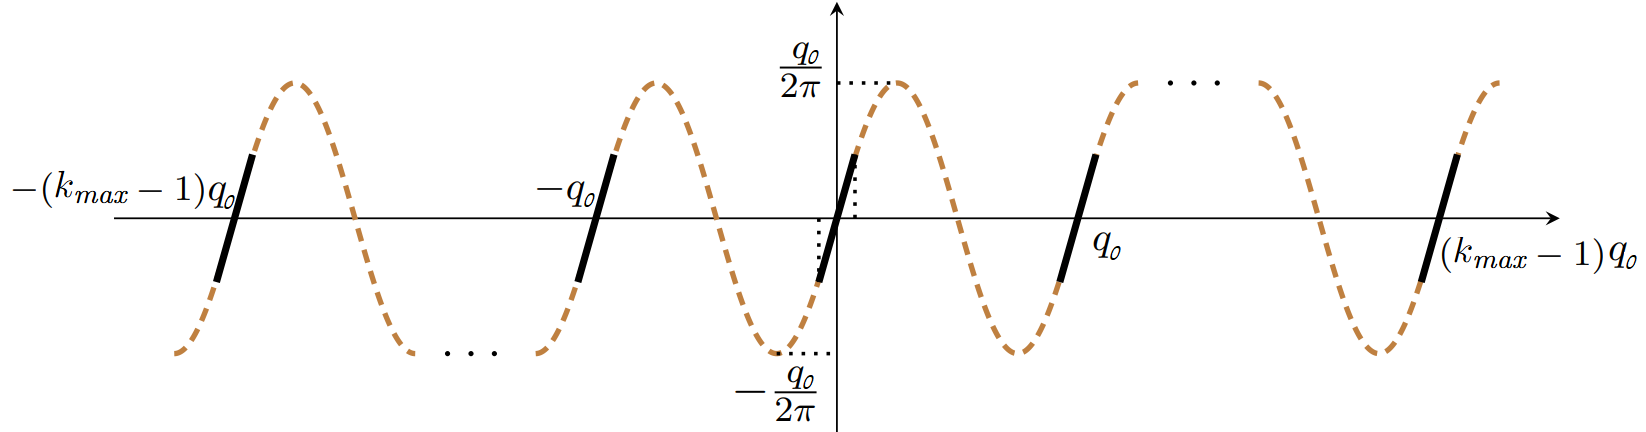
\includegraphics[width=1.0\linewidth]{figures/modulo-reduction-sine.png}
  \caption{Sine function $f(x) = \dfrac{q_0}{2\pi}\cdot \sin \left(\dfrac{2\pi x}{q_0}\right)$ such that $f(\Delta m_i + e_i + q_0k_i) \approx \Delta m_i + e_i$ (provided $\Delta m_i + e_i \ll q_0$) \href{https://eprint.iacr.org/2018/153.pdf}{(Source)}}
  \label{fig:modulo-reduction-sine}
\end{figure}

 To do so, we will take an approximated approach by using a sine function described in \autoref{fig:modulo-reduction-sine}, which has a period of $q_0$ with the amplitude $\dfrac{q_0}{2\pi}$. This sine function has the following two useful properties:
 
 \begin{enumerate}
\item When $f(x)$ is evaluated at $x$ values near the multiple of $q_0$, the result approximates to that of a line function $y = x$. This is because the derivative (slope) of $\sin x$ is $y' = \cos x$, and if $x$ is a multiple of $2\pi$, the slope is: $y' = \cos 2\pi = 1$. 
\item The evaluation of $f(x)$ eliminates the multiples of $q_0$ from the input (i.e., modulo reduction $q_0$)
\end{enumerate}

$ $

Combining these two properties, given input $x = \Delta m_i + e_i + q_0k_i$, 

$f(\Delta m_i + e_i + q_0k_i) = \dfrac{q_0}{2\pi}\cdot \sin \left(\dfrac{2\pi \cdot (\Delta m_i + e_i + q_0k_i))}{q_0}\right) = \dfrac{q_0}{2\pi}\cdot \sin \left(\dfrac{2\pi \cdot (\Delta m_i + e_i))}{q_0}\right) \approx \Delta m_i + e_i$

$ $


, provided $\Delta m_i + e_i$ is very close to 0 relative to $q_0$ (i.e., $\Delta m_i + e_i \ll q_0$). This is true, because by construction of the CKKS scheme, the plaintext modulus (even with scaling it up by $\Delta$), is significantly smaller than the ciphertext modulus. Therefore, to remove $q_0K$ from $\Delta M + E + q_0K$, we can update each coefficient of the polynomial $\Delta M + E + q_0K$ by evaluating it with the $f(x)$ sine function. However, we cannot directly update the coefficients of the polynomial, because the CKKS scheme (the RLWE scheme in general) only supports the input vector's slot-wise $(+, \cdot)$ operations. Therefore, to update the polynomial coefficients, we need to express the update logic in terms of slot-wise input vector arithmetic $(+, \cdot)$. Considering all these, CKKS's overall bootstrapping procedure is described in \autoref{tab:ckks-bootstrapping-procedure}.

\begin{table}
\begin{tabular}{|ll|}
\hline
1& \textsf{\textbf{\underline{ModRaise:}}} Given ciphertext $(A, B) \bmod q_L$, we forcibly modify its modulus from $q_0$ to $q_L$. \\
& Then, it ends up encrypting $\Delta M + E + q_0k$ instead of $\Delta M + E$.\\
2& \textsf{\textbf{\underline{CoeffToSlot:}}} Based on step 1's ciphertext $(A, B) \bmod q_L$, we generate a new ciphertext\\
& that encrypts an input vector whose its each $i$-th slot stores $\Delta m_i + e_i + q_0k_i$.\\
& This is equivalent to moving the coefficients of polynomial $\Delta M + E + q_0K$ to\\
& the input vector slots.\\
3& \textsf{\textbf{\underline{EvalExp:}}} We convert the sine function into an approximated polynomial by using \\
& the Taylor series, as well as other optimizations such as\\ 
& Euler's formula ($e^{i\theta} = \cos(\theta) + i\cdot\sin(\theta)$). Then, we generate a CKKS plaintext that encodes \\
& this approximated sine function, and then use this to homomorphically evaluate \\
& step 2's encrypted vector elements (to homomorphically remove every $q_0k_i$.\\
4& \textsf{\textbf{\underline{SlotToCoeff:}}} Based on the resulting ciphertext from step 3, we generate a new ciphertext \\
& whose encrypted polynomial's each $i$-th coefficient is (approximately) $\Delta m_i + e_i$. \\
& This is equivalent to moving the $q_0k_i$-eliminated values stored in the input vector slots in \\
&step 3 back to the positions of the polynomial coefficients. The final ciphertext is \\
& our goal ciphertext that (approximately) encrypts $\Delta M + E$ under modulus $q_L$.\\
\hline
\end{tabular}
\caption{High-level Description of CKKS's Bootstrapping Procedure}
\label{tab:ckks-bootstrapping-procedure}
\end{table}
%CKKS's bootstrapping procedure described above breaks down into the following 5 steps: \textsf{ModRaise}, \textsf{CoeffToSlot}, \textsf{EvalExp}, \textsf{ImgExt}, and \textsf{SlotToCoeff}.

\subsubsection{Mathematical Expansion of the High-level Idea}
\label{subsubsec:ckks-bootstrapping-high-level-correctness}

We will mathematically walk through how the bootstrapping procedure (\autoref{tab:ckks-bootstrapping-procedure}) correctly updates the modulus of the input ciphertext from $q_0$ to $q_L$. 

For ease of understanding, we will first explain how we would do modulus bootstrapping for a ciphertext with multiplicative level 0 (i.e., its modulus is $q_0$) in case we have access to the secret key $S(X)$. Using this key, we can decrypt the ciphertext as follows:

$\textsf{RLWE}^{-1}\textbf{(}\textsf{ct} = (A, B)\textbf{)}$ \textcolor{red}{ \# where $\textsf{ct}=(A, B) = \textsf{RLWE}_{S, \sigma}\bm(\Delta M \bm)$}

$ = B + A\cdot S = \Delta M + E \bmod q_0$ 

$ = \Delta M + E + q_0K$ \textcolor{red}{\# where $q_0K$ accounts for any potential wrap-around modulo $q_0$ values}

Our initial goal is to bootstrap the modulus of the ciphertext from $q_0$ to $q_L$ by using only the following three tools:

\begin{itemize}
\item Secret key $S$
\item Batch-encoding ($\sigma^{-1}$) and decoding ($\sigma$) formulas
\item Batched slot-wise $(+, \cdot)$ operation of input vectors based on their batch-encoded polynomials
\end{itemize}

$ $

After explaining the above, we will then explain how to achieve the same bootstrapping without having access to the secret key $S$. 


$ $

\para{\textsf{\textbf{\underline{ModRaise}:}}} This step forcibly changes the ciphertext's modulus from $q_0$ to $q_L$ and then decrypts the ciphertext as follows:

$\textsf{RLWE}^{-1}\textbf{(}\textsf{ct} = (A, B)\textbf{)} = B + A\cdot S = \Delta M + E + q_0 K \bmod q_L$

Notice that the ciphertext's decrypted plaintext polynomial's each $i$-th coefficient gets corrupted to $m_i + e_i + q_0\cdot k_i \bmod q_L$. So, we now need to eliminate the garbage term $q_0k_i \bmod q_L$ in each coefficient and distill the pure plaintext coefficient $\Delta m_i + e_i$. 

$ $

\para{\textsf{\textbf{\underline{CoeffToSlot}:}}} This step generates a new plaintext polynomial whose each $i$-th input vector slot stores the corrupted coefficient $(m_i + e_i + q_0k_i)$. The trick of doing this is to apply CKKS's batch-encoding mapping $\sigma^{-1}$ (which represents the transformation $\vec{m} = \dfrac{\hathat W \cdot I_n^R \cdot \vec{v}_{'}}{n}$ as explained in \autoref{subsec:ckks-encoding-decoding}) to the input vector slots that encode the polynomial $\Delta M + E + q_0 K \bmod q_L$. Let $\vec{v}_c$ be the input vector that corresponds to polynomial $\Delta M + E + q_0 K$. Then, $\vec{v}_c$ and $\Delta M + E + q_0 K$ satisfy the following relation over the encoding mapping $\sigma^{-1}$: 

$\sigma^{-1}\bm(\vec{v}_c\bm) = M_c = \sum\limits_{i=0}^{n-1}(\Delta m_i + e_i + q_0k_i)\cdot X^{i}$ \textcolor{red}{ \# i.e., polynomial $\Delta M + E + q_0K$} 

This implies that if we \textit{homomorphically} apply the $\sigma^{-1}$ transformation to the elements of input vector $\vec{v}_c$, then the resulting input vector $\vec{v}_s$ will store $\vec{v}_c$'s encoded polynomial coefficient values as follows:

$\sigma^{-1} \circ \vec{v}_c = \vec{v}_s = (\Delta m_0 + e_0 + q_0k_0, \text{ } \Delta m_1 + e_1 + q_0k_1, \text{ } \cdots, \text{ } \Delta m_{n-1} + e_{n-1} + q_0k_{n-1})$  

\textcolor{red}{ \# where $\circ$ represents a linear transformation operation comprising $(+, \cdot)$}

$ $




However, remember that at the end of the \textsf{ModRaise} step, we get the decrypted (but corrupted by $q_0k$) polynomial $M_c = \textsf{RLWE}^{-1}\textbf{(}\textsf{ct} = (A, B)\bm) = \Delta M + E + q_0K$ and we are not allowed to decode it into $\vec{v}_c$. Therefore, we will instead \textit{encode} the matrix $\hathat W \cdot I_n^R$ in the encoding transformation $\sigma^{-1}$ ($\vec{m} = \dfrac{\hathat W \cdot I_n^R \cdot \vec{v}_{'}}{n}$) into its equivalent polynomials (treating a matrix as a combination of vectors) and then perform batched slot-wise $(+, \cdot)$ operation between $M_c$ and the polynomial version of $\hathat W \cdot I_n^R$. We express this polynomial-based computation as follows:

$M_s = \sigma^{-1}_{\sigma^{-1}} \circ M_c \bmod q_L$
\textcolor{red}{ \# $\sigma^{-1}_{\sigma^{-1}}$ is the polynomial-encoded version of the $\sigma^{-1}$ transformation}

Then, the resulting polynomial $M_s$'s corresponding input vector slots (i.e., the decoded version of $M_s$) will store $\vec{v}_s = (\Delta m_0 + e_0 + q_0k_0, \text{ } \Delta m_1 + e_1 + q_0k_1, \text{ } \cdots, \text{ } \Delta m_{n-1} + e_{n-1} + q_0k_{n-1})$. In other words, the above computation effectively \textit{moves} the coefficients of $M_c$ to the input vector slots of a new plaintext polynomial. 

However, remember that in CKKS, an input vector can store only up to $\dfrac{n}{2}$ slots, whereas we need to store a total of $n$ coefficients of $M_c$ in the input vector slots. Therefore, we technically need to create 2 pieces of $M_s$ as $M_{s1}$ and $M_{s2}$, where the input vector of $M_{s1}$ stores $(\Delta m_0 + e_0 + q_0k_0, \text{ } \Delta m_1 + e_1 + q_0k_1, \text{ } \cdots, \text{ } \Delta m_{\frac{n}{2}-1} + e_{\frac{n}{2}-1} + q_0k_{\frac{n}{2}-1})$, and the input vector of $M_{s2}$ stores $(\Delta m_{\frac{n}{2}} + e_{\frac{n}{2}} + q_0k_{\frac{n}{2}}, \text{ } \cdots, \text{ } \Delta m_{n-1} + e_{n-1} + q_0k_{n-1})$.

$ $

\para{\textsf{\textbf{\underline{EvalExp}:}}}
Our next step is to update $\vec{v}_s$'s each element $m_i + e_i + q_0k_i$ to $m_i + e_i$ by evaluating it with the sine function $f(x)$. Since the output of the \textsf{CoeffToSlot} step is polynomial $M_s$ (technically $M_{s1}$ and $M_{s2}$), we need apply the evaluation transformation in an encoded form. First, we approximate $f(x)$ as linear combination comprising only $(+, \cdot)$ operations by using the Taylor series and Euler's formula (will be explained later). Then, we encode (i.e., $\sigma$) the approximated formula into a polynomial form, and we denote as $\sigma_f$. Finally, We apply the $\sigma_f$ transformation to $M_s$ as follows: 

$\sigma^{-1}_f \circ M_s \bmod q_L$  \textcolor{red}{ \# Applying the sine function's linear transformation to $\vec{v}_s$'s each slot storing $\Delta m_i + e_i + q_0k_i$}

$= M_t = \sigma\bm{(}\vec{v}_t\bm{)} = \sigma\bm{(}(\Delta m_i + e_i)_{i=0}^{n-1}\bm{)} \bmod q_L$

$ $

After the linear transformation by the sine function, notice that each $q_0 k_i$ term gets eliminated from $\vec{v}_s$'s slots (i.e. modulo reduction by $q$) and the resulting vector $\vec{v}_t$ stores only the $\Delta m_i + e_i$ terms. 

